\documentclass[a4paper, 11pt, oneside]{book}

\usepackage{fontspec}   %加這個就可以設定字體
\usepackage{xeCJK}       %讓中英文字體分開設置
\usepackage{indentfirst}
\usepackage{listings}
\usepackage{float}
\usepackage{graphicx}
\usepackage{caption}
\usepackage{fancyhdr}
\usepackage{hyperref}
\usepackage{amsmath}
\usepackage{multirow}
\usepackage{graphicx}
\usepackage{tabularx}
\usepackage{etoolbox}
\usepackage[newfloat]{minted}
\usepackage[dvipsnames]{xcolor}
\usepackage[breakable, listings, skins, minted]{tcolorbox}

\usepackage[
  margin=2cm,
  headheight=17pt, % as per the warning by fancyhdr
  includehead,includefoot,
  heightrounded, % to avoid spurious underfull messages
]{geometry} 

\hypersetup{
    colorlinks=true,
    linkcolor=black,
    filecolor=magenta,      
    urlcolor=blue,
} % 超連結顏色


\renewtcblisting{minted}{%
    listing engine=minted,
    minted language=cpp,
    listing only,
    breakable,
    enhanced,
    minted options = {
        linenos, 
        breaklines=true, 
        breakbefore=., 
        % fontsize=\footnotesize, 
        numbersep=2mm
    },
    overlay={%
        \begin{tcbclipinterior}
            \fill[gray!25] (frame.south west) rectangle ([xshift=4mm]frame.north west);
        \end{tcbclipinterior}
    }   
} % 程式碼片段

\pagestyle{fancy}

\newenvironment{code}{\captionsetup{type=listing}}{}
\SetupFloatingEnvironment{listing}{name=程式碼}

\renewcommand{\figurename}{圖}
\renewcommand{\chaptermark}[1]{\markboth{#1}{}}

\lhead{\chaptername~\thechapter}
\rhead{\leftmark}

\cfoot{\thepage}


\setCJKmainfont{Noto Sans CJK TC} % 中文主字體
\setmonofont{CascadiaCode.ttf}    % 等寬字體 (用於程式碼)
% \setmonofont{Consolas}
\XeTeXlinebreaklocale "zh"             %這兩行一定要加,中文才能自動換行
\XeTeXlinebreakskip = 0pt plus 1pt     %這兩行一定要加,中文才能自動換行
\title{武陵資訊讀書會講義} 
\author{李杰穎}
\date{\today}

\setlength{\parindent}{2em} % 句首縮排兩字元
\setlength{\parskip}{0.5em} % 段落間0.5字元

\renewcommand{\baselinestretch}{1.5} % 行距=1.5倍行高
\newcommand{\wlojURL}{http://wloj.wlsh.tyc.edu.tw/} 

\begin{document}
\maketitle
\tableofcontents

\chapter{前言}
\section{課程介紹}
先來介紹一下資訊讀書會吧!

資訊讀書會是去年 (2019) 才新成立的讀書會。我們上學期會教C++的語法/演算法,而下學期主要是C++算法的加強及一些如何做專題的技巧。下學期也有可能會用Python和PyTorch來上一點人工智慧的部份。課表部份未來應該會公佈在課程網站上。

前面兩堂課主要是上最基礎的語法,所以我們會採用發講義的形式讓大家可以看著講義練習寫寫看題目。當然,講師會先把講義內容清楚的帶過一次在讓你們寫練習題。如果在寫練習題的過程中有遇到困難也可以詢問各個講師。

\section{編輯器/IDE(整合式開發環境)介紹}
\begin{itemize}
    \item \href{https://sourceforge.net/projects/orwelldevcpp/}{\underline{Dev-C++}}:應該算IDE。安裝好後就可以直接使用,不需額外安裝編譯器或擴充功能。缺點是不能自動補程式碼(autocomplete),但主要還是推薦使用這個編輯器啦。
    \item \href{https://sourceforge.net/projects/codeblocks/files/Binaries/20.03/Windows/codeblocks-20.03-setup.exe/download}{\underline{Code::Blocks}}:功能比Dev-C++完整的IDE。Autocomplete是好的,可以用。整體而言有點太肥了,所以我不太常用。不過還是一個不錯的選擇拉。
    \item \href{https://code.visualstudio.com/}{\underline{Visual Studio Code}}:微軟出的編輯器,本身的功能可以透過許多擴充功能(extensions)進行擴充。如果想要在VS Code上寫C++就要裝C++的擴充功能才能比較方便的使用。經過一些設定後,autocomplete的功能十分強大,而且內建的terminal對於執行程式很方便。
    \item \href{https://notepad-plus-plus.org/}{\underline{NotePad++}}:超級威力加強板的windows內建筆記本,支援程式碼highlighting,啟動很快。如果專注在打code或驗測資之類的也可以考慮用這款。
    \item \textbf{其他 (Sublime Text, Eclipse IDE, vim, nano, emacs, far file manager...)}:一些在打competitive programming在用的編輯器 or IDE,有興趣可以去網路上找找看相關的資料。
\end{itemize}

大家可以慢慢嘗試,找出自己最喜歡的編輯器喔。



\section{課程網站及線上批改系統(Online Judge)}
\begin{itemize}
    \item \textbf{課程網站}(\url{https://wulinginfor.github.io/}):接下來上課的內容都會放在課程網站上,講義、投影片那些的都會放在上面,練習題也會公佈在上面。如果回家想要練習的話,就可以去網站上看看喔。
    \item \textbf{Online Judge}(\url{\wlojURL }(WLOJ)):如果有在刷題的人應該對這個名字不太陌生。Online Judge(或簡稱OJ)就是一個會有許多程式題目的網站,在每一題中,都有題目敘述、輸入、輸出,我們要做的就是寫一個程式滿足題目敘述,使當輸入輸進來時程式都可以得到正確的輸出。當你認為你已經把程式寫完了,就可以把原始碼上傳到網站上,網站經過批改後,就會告訴你的程式是不是好的(\textcolor{ForestGreen}{Accepted(AC)})或者是錯的(\textcolor{red}{Wrong Answer(WA)})或者是編譯錯誤(\textcolor{orange}{Compile Error(CE)})又或者程式是否超過了題目所限制的資源(時間、記憶體等)(\textcolor{orange}{Time Limit Exceeded(TLE), Memory Limit Exceeded(MLE)})
\end{itemize}

\section{教學資源}
\begin{itemize}
    \item \href{https://tw-csie-sprout.github.io/c2020/#!index.md}{\underline{2020資訊之芽語法班}}:資訊之芽語法班是台大和清大一起合開的課,在清大和台大都有開課。他們會把上課的內容全部丟到網路上讓有需要的人可以學習。
    \item \href{https://www.csie.ntu.edu.tw/~sprout/algo2020/}{\underline{2020 資訊之芽算法班}}:資訊之芽算法班是更為進階的課程,只有在台大開課。對算法班課程有興趣的人可以關注一下資訊之芽的粉絲專頁,他們每年大約寒假的時候就會有課程報名的消息了。
    \item \href{www.geeksforgeeks.org}{\underline{GeeksForGeeks}}:國外的網站,有很多語法和算法的教學,如果對某個語法或算法不熟可以上去找一下。
\end{itemize}
\section{Online Judge}
\begin{itemize}
    \item \href{https://neoj.sprout.tw/}{\underline{Sprout OJ}}:資訊之芽的OJ,上面有各種難度的題目,有興趣的可以刷刷看。
    \item \href{https://zerojudge.tw}{\underline{ZeroJudge}}:應該是台灣最大的OJ, 題目超級多,幾乎不可能刷完。水題偏多(至少前30題都滿水的),但還是有不錯的題目。
    \item \href{https://onlinejudge.org/}{\underline{UVa Online Judge}}:全世界第一個OJ,想當然爾題目非常的多。缺點是網站的界面有點不太直觀,但似乎準備要更新了。
    \item \href{https://codeforces.com}{\underline{CodeForces}}:全世界最大的線上程式競賽網站,題目相當有水準,如果上面的題目都解不出來也不要太挫折喔。
    \item \href{https://csacademy.com/}{\underline{CS Academy}}:CS Academy 上面有很多不錯的題目,而且每題都會分成Easy, Medium及Hard。大家可以看自己的解題情況決定要怎麼刷題喔。
\end{itemize}


\chapter{Hello World!}
\begin{code}
    \captionof{listing}{一個標準的C++程式碼}
    \begin{minted}
#include <iostream>
using namespace std;
int main(){
    cout << "Hello World!" << endl;
    return 0;
}
\end{minted}
\end{code}

大家可以把這段code複製到Dev C++上。

想必大家在學習各種程式語言的第一個程式應該都是Hello World吧。資訊讀書會也不例外,我們就來看看這段程式碼在寫什麼吧。

第一行是引入C++的輸入輸出標頭檔(header file),如果沒有引入這個標頭檔,C++程式就沒有辦法在程式執行的畫面(小黑窗)上輸出或輸入東西了,也就看不到程式的執行過程了。

第二行對於目前來講不太重要啦,下面是如果不加這行code,一個能成功編譯的code會長怎樣。
\begin{code}
    \captionof{listing}{一個標準的C++程式碼但不加\texttt{using namespace std}}
    \begin{minted}
#include <iostream>
int main(){
    std::cout << "Hello World!" << std::endl;
    return 0;
}
\end{minted}
\end{code}

可以發現如果不加這行,\texttt{cout}跟\texttt{endl}前面就要再加上\texttt{std::},實際寫程式的時候變得相當的麻煩,所以一般來說在寫C++的時候多會在\texttt{\#include}下面加上這行。

第三行是一個特別的函數(function),我們稱之為main function,它是整段C++程式開始執行的進入點,C++的執行都會從這個函數開始。至於\texttt{int main() \{ ...  \}}是什麼意思我們以後會提到。

第四行就是整段程式輸出 Hello World! 的地方,主要由\texttt{cout, <<, endl} 組成,大家可以把 \texttt{cout} 想成用來處理輸出的關鍵字(keywords),我們用 \texttt{<<} 來把我們要輸出的文字 (字串) 括起來,而\texttt{endl} (endline)則是用來換行的,大家可以試試看如果把\texttt{endl}刪掉會發生什麼事。

第五行是整個main function的終止點。一般來說,如果main function有成功執行的話,其回傳值就是0。至於回傳值是什麼我們也等到以後再提吧。

\section{練習題}
\begin{itemize}
    \item \href{\wlojURL problem/1001}{\underline{WLOJ 1001: Hello World!}}
\end{itemize}

\chapter{表達式與變數}
\begin{code}
    \captionof{listing}{解一元二次方程式}
    \begin{minted}
#include <iostream>
#include <cmath>

using namespace std;

int main(){
    // ax^2 + bx + c = 0
    double a, b, c;
    cin >> a >> b >> c;
    cout << (-b+sqrt(b*b-4*a*c))/(2*a) << " ,";
    cout << (-b-sqrt(b*b-4*a*c))/(2*a) << endl;
    return 0;
}
\end{minted}
\end{code}
在這段code中,我們多引入了一個標頭檔cmath,引入這個標頭檔可以讓我們使用sqrt()這個函數,sqrt是square root的縮寫,也就是開根號。有了根號我們就可以利用公式解,解出一元二次方程式的兩個根。

\section{合法的程式}
\begin{itemize}
    \item 標頭檔(header file): \\
          標頭檔像是指令的說明書。特定功能要在特定的說明書中才會描述。所以當使用不同函數時,可能要引入不同的標頭檔。
    \item 主函式 (main function): \\
          顧名思義,主程式。程式由此開始執行。
\end{itemize}
\section{輸入輸出}
在C++中,我們通常使用cin、cout來處理輸入、輸出。使用這兩個功能需要引入標頭檔iostream,也要記得打using namespace std;

\begin{itemize}
    \item \texttt{cout} (念see-out) 代表輸出
    \item \texttt{cin} (念see-in) 代表輸入
    \item 注意\texttt{cout}、\texttt{cin}的箭頭方向是相反的(\texttt{<< (cout)、>> (cin)}),可以想像成資料的流向
    \item \texttt{<<、>>} 裡面的東西會被解讀成字或特殊符號
    \item 最後記得加分號,代表敘述句結束
\end{itemize}

\section{運算子}
運算子是C++用來進行數學運算的符號,C++除了能做到基本的加減乘除外,還可以做到許多特殊的運算。

下面是一些常見的運算子 (按運算優先級排列):
\begin{itemize}
    \item \texttt{++}:遞增, \texttt{i++}
    \item \texttt{--}:遞減, \texttt{i--}
    \item \texttt{[]}:陣列存取, \texttt{a[1]}
    \item \texttt{!}:邏輯非(not), \texttt{!a}
    \item \texttt{*}:就是乘號
    \item \texttt{/}:就是除號
    \item \texttt{\%}:取餘數
    \item \texttt{+}:就是加號
    \item \texttt{-}:就是減號
    \item \texttt{>>}:位元右移, \texttt{a >> 1}
    \item \texttt{<<}:位元左移, \texttt{a << 1}
    \item \texttt{>}:大於關係, \texttt{3 > 2} (運算結果\texttt{true})
    \item \texttt{>=}:大於等於關係, \texttt{3 >= 3} (運算結果\texttt{true})
    \item \texttt{<}:小於關係, \texttt{3 < 2} (運算結果\texttt{false})
    \item \texttt{<=}:小於等於關係, \texttt{3 <= 3} (運算結果\texttt{false})
    \item \texttt{==}:等於關係, \texttt{3 == 3} (運算結果\texttt{true})
    \item \texttt{!=}:不等於關係, \texttt{3 != 3} (運算結果\texttt{false})
    \item \texttt{\&\&}:邏輯 AND, \texttt{true \&\& false} (運算結果\texttt{false})
    \item \texttt{||}:邏輯 OR, \texttt{true || false} (運算結果\texttt{true})
    \item \texttt{=}:直接賦值
    \item \texttt{+=}:以和賦值, \texttt{a = 1, a += 2}, (\texttt{a}此時為3) (等價於\texttt{a = a + 2})
    \item \texttt{-=}:以差賦值
    \item \texttt{*=}:以積賦值
    \item \texttt{/=}:以商賦值
    \item \texttt{\%=}:以取餘數賦值
\end{itemize}

\section{表達式}
表達式是一種廣義的算式,代表一個\textbf{值}。每個表達式包含運算子和運算元,運算規則就是先乘除後加減,每個運算的優先度不同。

\begin{code}
    \captionof{listing}{各種表達式}
    \begin{minted}
(-b-sqrt(b*b-4*a*c)/(2*a) // 值由a, b, c的值決定
7122 % 20 // 取餘數運算,算出的值為2
0 < 3 // ⼩於運算, 算出的值為True,也就是1
6/2(1+2) // 少了乘號,編譯器看不懂
a*x*x + bx + c = 0 // 這是⽅程式,本⾝沒有值,編譯器看不懂
\end{minted}
\end{code}

\section{變數}
變數是程式中很重要的元素。程式中如果沒有變數就沒辦法達成很多我們想要達成的功能了。

在C++中,變數在使用前需要先宣告(declare)。與Python不同,C++的變數在宣告時就要決定這個變數的資料型態(等等會提到)。變數的名稱只能是英文或底線開頭,後面可以有數字,但不能是保留字(keywords, 後面應該會提到)。另外,大小寫對於變數的名稱是不同的。

變數可以讀,也可以改(const除外),變數的數值儲存在電腦的記題體中。讀值的時候直接當作數值使用。而寫值的時候通常使用等號來寫,這個等號是賦值(把一個數值給一個變數)的意思,與數學中的等號不同。通常我們把等號左邊稱作lvalue、右邊稱為rvalue。
\begin{code}
    \captionof{listing}{一堆變數}
    \begin{minted}
#include <iostream>
using namespace std;
int main(){
    int price = 8740;
    int my_money_Monday = 314159;
    int my_money_Tuesday = my_money_Monday - price;
    my_money_Monday = my_money_Monday - price*6; // 寫⼊
    my_money_Monday -= price * 7; // 偷懶的寫法
    cout << my_money_Monday * 1.0106 << endl;
    return 0;
}
\end{minted}
\end{code}

\begin{code}
    \captionof{listing}{不好的示範}
    \begin{minted}
#include <iostream>
using namespace std;
int main(){
    int my_money=59457, price=879457 // 沒有分號
    bool have_money, 1_thing_to buy=0; // 數字開頭、有空隔
    my_money <- (my_money - buy*price); // <- 不能給值,請⽤=
    have_Money = my_Money <> 0; // 沒有宣告(⼤寫)、不等於請⽤!=
    cin << price; // ⽅向錯
    cout << "我" < have_Money << "定不是沒錢\n"; // ⼩於?
    cout << yee~ << my_Money > 0; // 沒引號,>運算要加括號
    return 0;
}
\end{minted}
\end{code}

\section{變數的資料型態}
在C++中,變數被分為了很多不同的資料型態。資料型態有非常多種,甚至可以自己創一個資料型態,以下只列出最基礎的幾種。

\begin{table}[H]
    \begin{tabularx}{\linewidth}{|c|X|X|X|X|}
        \hline
        類型                           & 資料型態           & 名稱                & 佔有記憶體空間 (bytes) & 儲存值範圍                                              \\ \hline
        \multirow{5}{*}{整數}          & bool               & 布林                & 1                      & 0 $\sim$255                                             \\ \cline{2-5}
                                       & int                & 整數                & 4                      & $-2^{31} \sim 2^{31} - 1$                               \\ \cline{2-5}
                                       & unsigned int       & 無號整數 (無負數)   & 4                      & $0 \sim 2^{32} - 1$                                     \\ \cline{2-5}
                                       & long long          & 長整數              & 8                      & $-2^{63} \sim 2^{63} - 1$                               \\ \cline{2-5}
                                       & unsigned long long & 無號長整數 (無負數) & 8                      & $0 \sim 2^{64} - 1$                                     \\ \hline
        \multirow{3}{*}{浮點數 (小數)} & float              & 單精度浮點數        & 4                      & $\pm 3.4 \times 10^{-38} \sim \pm 3.4 \times 10^{38}$   \\ \cline{2-5}
                                       & double             & 倍精度浮點數        & 8                      & $\pm 1.7 \times 10^{-308} \sim \pm 1.7 \times 10^{308}$ \\ \cline{2-5}
                                       & long double        & 長倍精度浮點數      & 12$\sim$16             & $\pm 1.7 \times 10^{-308} \sim \pm 1.7 \times 10^{308}$ \\ \hline
        字元                           & char               & 字元                & 1                      & 0 $\sim$255                                             \\ \hline
    \end{tabularx}
\end{table}

有了這些資料型態,我們就可以在適當的時機使用特定資料型態的變數,來達成目標。

\section{練習題}
\begin{itemize}
    \item \href{\wlojURL problem/1002}{\underline{WLOJ 1002: A+B Problem}}
    \item \href{\wlojURL problem/1003}{\underline{WLOJ 1003: 球球的表面積}}
    \item \href{\wlojURL problem/1004}{\underline{WLOJ 1004: 我要成為化學大師}}
    \item \href{\wlojURL problem/1006}{\underline{WLOJ 1006: A+B Problem (Hard Version)}}
\end{itemize}
\chapter{流程控制 (if...else)}
\section{if}
if就是英文中如果的意思,在C++中,我們可以透過if來進行流程控制。具體直接看code吧。

\begin{code}
    \captionof{listing}{if}
    \begin{minted}
#include <iostream>
using namespace std;
int main(){
    if (1 * 2 >= 2){
        cout << "1 * 2 >= 2" << endl;
    }    
    cout << "statements after if" << endl;
}
\end{minted}
\end{code}
簡單來說,當if後面跟的那個括號那個敘述是true的話,程式就會執行大括號內的程式碼。

小提醒,如果你想要判斷一個數字x是否介於30跟60之間的話,判斷式不能寫成\texttt{30<=x<=60},要寫成\texttt{(30 <= x) \&\& (x <= 60)}。原因是因為\texttt{30<=x<=60}可以寫成\texttt{(30<=x)<=60},但\texttt{(30<=x)}可以是0或1,而0<=60,1<=60,所以不管x的值是多少這個敘述都是對的。
\section{else \& else if}
else就是英文中的不然的意思,else配合if就可以達到更完整的流程控制。else只能接在if後面,當if內的敘述不成立時,程式就會繼續往下看是否有else或else if。else與else if的差別在於else if後面也是跟著一個敘述,而else沒有敘述,當程式碰到else的時候,就會直接執行大括號裡面的程式碼。

\begin{code}
    \captionof{listing}{if, else if, else}
    \begin{minted}
#include <iostream>
using namespace std;
int main(){
    if (condition1) {
        cout << "I'm in condition1" << endl;
    } else if (condition2) {
        cout << "I'm in condition2" << endl;
    } else {
        cout << "I'm in else" << endl;
    }
}
\end{minted}
\end{code}

小提醒,在一段if, else if, else區段中,只有一個大括號會被程式執行。也就是說,當區段中已經有大括號內程式碼被執行的話,其他大括號內的程式碼是絕對不會被執行的到,就是其敘述是正確的。例如下面這段code。

\begin{code}
    \captionof{listing}{Never be executed}
    \begin{minted}
#include <iostream>
using namespace std;
int main(){
    if (true) {
        cout << "I will be executed." << endl;
    } else if (true) {
        cout << "I will never be executed QQ" << endl;
    }
}
\end{minted}
\end{code}
\section{練習題}
\begin{itemize}
    \item \href{\wlojURL problem/1005}{\underline{WLOJ 1005: 季節判斷}}
    \item \href{\wlojURL problem/1007}{\underline{WLOJ 1007: 3n+1 Problem (Easy Version)}}
    \item \href{\wlojURL problem/1008}{\underline{WLOJ 1008: 天將降大任於斯人也}}
\end{itemize}
\chapter{while 迴圈}
如果你現在想要把1$\sim$10的數字分別印出來的話,你會怎麼做呢?以下是其中一種方法:
\begin{code}
    \captionof{listing}{Naive 的作法}
    \begin{minted}
#include <iostream>
using namespace std;
int main(){
    cout << 1 << endl;
    cout << 2 << endl;
    cout << 3 << endl;
    cout << 4 << endl;
    cout << 5 << endl;
    cout << 6 << endl;
    cout << 7 << endl;
    cout << 8 << endl;
    cout << 9 << endl;
    cout << 10 << endl;
}
\end{minted}
\end{code}
看起來是不是有點繁瑣呢?但如果這時你又想要印出可能1$\sim$1000、1$\sim$10000的數字時,以上的作法就會變得非常的不好,程式沒辦法簡潔的寫出來。

此時,while迴圈就派上用場了,while迴圈具體會長這樣:
\begin{code}
    \captionof{listing}{while迴圈}
    \begin{minted}
#include <iostream>
using namespace std;
int main(){
    while(condition){
        // statements
    }
}
\end{minted}
\end{code}
while迴圈具體會做的事就是當conditon為true時,while迴圈就會執行大括號裡面的程式碼。但與if不同的是,當大括號裡面的程式碼執行完後,while迴圈會再一次的檢查condition是否仍然是true,如果是的話就繼續執行大括號內的程式碼,直到condition為false為止。

所以上面的code就可以改寫成這樣:
\begin{code}
    \captionof{listing}{while 迴圈的作法}
    \begin{minted}
#include <iostream>
using namespace std;
int main(){
    int n = 1;
    while (n <= 10){
        cout << n << endl;
        n ++;  // 與 n = n + 1 和 n += 1 相同
    }
}
\end{minted}
\end{code}

\section{do...while 迴圈}
除了一般的while迴圈以外,還有一種特殊的while迴圈,稱之為do...while迴圈,具體長這樣:
\begin{code}
    \captionof{listing}{do...while迴圈}
    \begin{minted}
#include <iostream>
using namespace std;
int main(){
    do{
        // statements
    } while(condition);
}
\end{minted}
\end{code}

可以發現在do...while迴圈中,出現了do這個關鍵字,且while的condition也放在了大括號的後面。do...while迴圈與while迴圈不同的地方在於do...while迴圈將先會執行一次大括號內的程式碼,再去判斷condition是否為true。所以無論condition是否為true,do-while迴圈大括號內的程式碼至少會執行一次。因此,do-while循環屬於後測迴圈 (post-test loop)。相對的,while迴圈就被稱為前測迴圈 (pre-test loop)。

一般來說,do...while迴圈很少被使用,除了以後會講到的\texttt{next\_permutation()}函數才會與do...while迴圈配合使用。

\section{練習題}
\begin{itemize}
    \item \href{\wlojURL problem/1009}{\underline{WLOJ 1009: 3n+1 Problem (Hard Version)}}
    \item \href{\wlojURL problem/1010}{\underline{WLOJ 1010: 階乘問題}}
    \item \href{\wlojURL  problem/1011}{\underline{WLOJ 1011: 武陵專用拖鞋}}
\end{itemize}

\section{break \& continue}
\subsection{break}
當在迴圈中,如果你突然不想讓迴圈繼續執行接下來的程式碼的話,我們就可以加上一行\texttt{break;},使迴圈直接跳出,不繼續執行接下來的程式碼,具體而言在while迴圈中的使用如下:
\begin{code}
    \captionof{listing}{break}
    \begin{minted}
#include <iostream>
using namespace std;
int main(){
    while(condition){
        // some statements
        break;
        // this part of statements will never be executed
    }
}
\end{minted}
\end{code}
可以發現由於break的特性,break通常與if一起配合使用。也就是說讓迴圈控制在一定條件才會跳出。

\subsection{continue}
另一個與while迴圈配合使用的是continue,它的功能和break有點類似,都是使程式不會執行到在它下面的程式碼。但與break不同的是,continue並不會跳出迴圈,而是繼續執行迴圈,只不過使它以下的程式碼不會被執行而已。
\begin{code}
    \captionof{listing}{continue}
    \begin{minted}
#include <iostream>
using namespace std;
int main(){
    while(condition){
        // some statements
        continue;
        // this part of statements will never be executed, 
        // but the rest of statements will be executed continuously.
    }
}
\end{minted}
\end{code}
同樣的,continue也常跟if一起搭配使用。

break和continue都是我們所謂的關鍵字(keywords),這些關鍵字在程式中佔有重要的位置。
\chapter{for 迴圈}
有了while迴圈,所以需要迴圈才能做到的事似乎就迎刃而解了。但事情可沒想像的那麼簡單,我們來看看下面這個例子,假設你現在想要重複做一件事 (執行一段程式碼) 10次,在while迴圈大概就要這樣寫:
\begin{code}
    \captionof{listing}{用while迴圈來重複做事}
    \begin{minted}
#include <iostream>
using namespace std;
int main(){
    int i = 0;
    while(i < 10){
        // some statements
        i ++;
    }
}
\end{minted}
\end{code}
有沒有覺得很麻煩呢?變數的初始化、判斷式、變數的累加被分到了三行,感覺就一整個不對了,所以程式設計師很聰明的設計出了for 迴圈,上面的程式碼就可以被縮減成這樣:
\begin{code}
    \captionof{listing}{用for迴圈來重複做事}
    \begin{minted}
#include <iostream>
using namespace std;
int main(){
    for(int i=0;i<10;i++){
        // some statements
    }
}
\end{minted}
\end{code}
有沒有覺得看起來簡短很多呢?變數(計數器)的初始化、判斷式、變數的累加全部被縮到了一行,而且很好的是,在for 迴圈中宣告的變數生命週期(lifetime)只有在for迴圈中(生命週期以後會提到),這當然包括了這裡的\texttt{int i}變數,所以我們就可以在這個for迴圈後,重複使用\texttt{int i}變數,而不會出現重複宣告的問題。下面是for 迴圈的具體使用方法。
\begin{code}
    \captionof{listing}{for迴圈}
    \begin{minted}
#include <iostream>
using namespace std;
int main(){
    for(initialization;condition;afterthought){
        // some statements
    }
}
\end{minted}
\end{code}
for迴圈的括號內主要包含三個部分:初始化(initialization)、條件式(condition)和遞增(afterthought),\textbf{值得注意的是這三個部分是由分號\texttt{;}來做分割的},並不像函數是用逗號\texttt{,}來做分割的,這點是需要注意的,如果不小心寫錯就會無法編譯成功了。

初始化是宣告(或者賦值)任何需要的變數的動作。如果你要使用多個變數,則變數的種類要一致。條件的部分則是檢查是否需要跳出for迴圈。如果條件為true,則繼續執行迴圈。如果條件判斷為false,則離開迴圈。遞增在每跑一次迴圈都會重複執行一次。

for 迴圈的三個部分是可有可無的,也就是說,我們其實可以將for迴圈當作無窮迴圈使用:
\begin{code}
    \captionof{listing}{for無窮迴圈}
    \begin{minted}
#include <iostream>
using namespace std;
int main(){
    for(;;){
        // some statements
    }
}
\end{minted}
\end{code}

\section{巢狀for迴圈}
我們可以在for迴圈中,再加上一個for迴圈,具體會長這樣:
\begin{code}
    \captionof{listing}{for巢狀迴圈}
    \begin{minted}
#include <iostream>
using namespace std;
int main(){
    int x, y;
    for(int i=0;i<x;i++){
        for(int j=0;j<y;j++){
            // some statements
        }
    }
}
\end{minted}
\end{code}

可以想一下這個巢狀迴圈內的statements總共會執行幾次?

同樣的,我們也可以在for迴圈中使用break/continue,其效果與while迴圈中相同。

\section{for迴圈與while迴圈的比較}

\begin{itemize}
    \item for迴圈和while迴圈可以互相轉換,主要視情況使用。
    \item 一般來說,for迴圈主要是用於當迴圈要跑的次數是固定時或每次跑完迴圈都要有固定的更新。
    \item 反之,若迴圈執行次數較不明確,或條件牽扯到使用者輸入,則適合使用while迴圈。
\end{itemize}

條件牽扯到使用者輸入,例如當輸入是由EOF(End of File)做結尾時,就適合使用while迴圈進行輸入的處理:

\begin{code}
    \captionof{listing}{\texttt{while(cin >> n)}}
    \begin{minted}
#include <iostream>
using namespace std;
int main(){
    int n;
    while(cin >> n){
        // some statements to deal with inputs
    }
}
\end{minted}
\end{code}
這個程式碼為甚麼可以偵測到EOF呢?原因是因為當\texttt{cin}偵測到現在讀入到EOF時,\texttt{cin >> n}就會因為沒辦法正確的讀取到一個整數而回傳false(反之正常情況下,\texttt{cin >> n}都會回傳true),所以當\texttt{cin}讀到一個整數的時候,就會直接跳出while迴圈,輸入部分也跟著處理完成,就可以開始進行題目需要做的運算。

\chapter{Coding/Programming Style}
我覺得這份2020資訊之芽語法班的簡報寫的很好,可以去看看:\url{https://www.csie.ntu.edu.tw/~b06902029/reveal.js/Sprout/2020/CodingStyle},以下是一些簡報裡面提到的重點:

\begin{itemize}
    \item \textbf{大準則:}
          \begin{itemize}
              \item 可讀性 (Readability Counts)
              \item 前後一致 (Be Consistent)
              \item \textbf{想想自己五年後還看不看得懂這份code}
          \end{itemize}
    \item \textbf{變數命名:}
          \begin{itemize}
              \item 一定要有它的意義,避免無意義的變數:
                    \begin{itemize}
                        \item O: \texttt{numOfStudents, num\_of\_students}
                        \item X: \texttt{a, b, ..., tmp}
                    \end{itemize}
              \item 可以使用一些縮寫、命名慣例:
                    \begin{itemize}
                        \item 縮寫:\texttt{number}  $\rightarrow$ \texttt{num, length} $\rightarrow$ \texttt{len}
                        \item 命名慣例:迴圈中的\texttt{i, j, k}
                    \end{itemize}
              \item 變數的命名若是由多個詞組合而成,主要可以使用兩種方式進行串接:
                    \begin{itemize}
                        \item \textbf{camelCase: }
                              \begin{itemize}
                                  \item 直接把多個詞串在一起。第一個字字首不大寫,其他字字首皆大寫。
                                  \item 如\texttt{numOfStudents}
                              \end{itemize}
                        \item \textbf{under\_score: }
                              \begin{itemize}
                                  \item 全部小寫,兩字中間用底線\texttt{\_}串連。
                                  \item 如\texttt{num\_of\_students}
                              \end{itemize}
                    \end{itemize}
          \end{itemize}
    \item \textbf{程式長相:}
          \begin{itemize}
              \item 縮排:
                    \begin{itemize}
                        \item 縮排很重要,沒有縮排沒人會想幫你debug。
                        \item 通常進入一個大括號縮排一次。
                        \item 注意縮排的格數要一致,沒有一致跟沒縮一樣。
                    \end{itemize}
              \item 空格:
                    \begin{itemize}
                        \item 適時加上空格可以增加可讀性。
                        \item \texttt{int k = a * b + c;} $>$ \texttt{int k=a*b+c;}
                        \item \texttt{cout << some << thing << endl;}
                    \end{itemize}
              \item 註解:
                    \begin{itemize}
                        \item 適時加上註解
                              \begin{itemize}
                                  \item \texttt{//}:單行註解
                                  \item \texttt{/* ... */}:區塊註解
                              \end{itemize}
                        \item 註解盡量使用 \href{https://zh.wikipedia.org/zh-tw/ASCII}{\underline{ASCII}}
                    \end{itemize}
          \end{itemize}
\end{itemize}

\chapter{陣列}
\section{1000根棍子}
假設你是某個工廠的老闆,今天工廠生產了1000根棍子,編號分別是1$\sim$	1000,而且每根棍子都有不同的高度。

這時有一位員工的工作是把編號1的棍子和編號1000的棍子接起來、編號2的棍子和編號999的裩子接起來、...、編號$n$和編號$1001-n$的棍子接起來。但是因為要趕著出貨的關係,所以你想要在這位員工還沒把棍子接起來前就知道這500根棍子的長度了。

如果這時你不會陣列的話,把上面的任務寫成程式大概會長這樣:\url{https://ideone.com/MZnVgd}

非常的慘,所以這時候應該要怎麼做呢?

\section{一維陣列}
甚麼是陣列(array)呢?簡單來說就是把有相同性質的資料連接起來,且這些連接起來的資料可以使用索引(index)來存取,具體可以看code:
\begin{code}
    \captionof{listing}{陣列(array)}
    \begin{minted}
#include <iostream>
using namespace std;
int main(){
    int s[4];
    cin >> s[0] >> s[1] >> s[2] >> s[3];
    cout << s[0] + s[3] << endl;
    cout << s[1] + s[2] << endl;
}
\end{minted}
\end{code}
\subsection{宣告}
首先看到main function的第一行,這行就是宣告陣列的地方,宣告的方式則是\\``資料型態\ 陣列名稱[陣列大小]",所以在上述的程式碼中,我們在第一行就宣告了一個``長度為4(代表陣列中有4個變數)的整數s陣列"。

\subsection{存取}
再來是第二行的部分,這邊主要就是存取陣列內的變數,我們可以透過在方括號中填入索引值(index)來存取變數,要注意的是在C++中,\underline{陣列的第一個變數(元素)的索引值為0},這點非常重要,很多初學者都會不小心忘記這點。所以在上述變數中,如果試著存取\texttt{s[4]}就會使程式無法順利的執行下去,可能會出現Runtime Error或甚至在編譯期間就不給過了。

\subsection{初始化}
C++中,陣列的初始化有幾種作法,具體如下:
\begin{code}
    \captionof{listing}{陣列的初始化}
    \begin{minted}
#include <iostream>
using namespace std;
int main(){
    int Sa[5] = {0, 1, 2, 3, 4};
    int Sb[5] = {0, 1}; // 自動補零
    int Sc[] = {0, 1, 2, 3, 4, 5, 6, 7}; //自動計算長度
    int Sd[1000000] = {}; // 全部補零,因為會自動補零
}
\end{minted}
\end{code}
大家可以試著編譯看看,然後陣列裡面的某個變數,看看裡面放了甚麼。

所以上面的1000根棍子問題就可以很簡單的解決了,具體的code如下:
\begin{code}
    \captionof{listing}{1000根棍子}
    \begin{minted}
#include <iostream>
using namespace std;
int main(){
    int s[1000];
    for(int i=0;i<1000;i++){
        cin >> s[i];
    }
    for(int i=0;i<500;i++){
        cout << s[i] + s[999 - i] << endl;
    }
}
\end{minted}
\end{code}

\subsection{不標準寫法}

\begin{code}
    \captionof{listing}{不標準寫法}
    \begin{minted}
#include <iostream>
using namespace std;
int main(){
    int n;
    cin >> n;
    int arr[n] = {};
    return 0;
}
\end{minted}
\end{code}

ㄟ感覺滿對的喔,然後丟到Dev-C++編譯也是對的,這有甚麼錯呢?其實在C++的標準中,陣列長度內放變數是不正確的,有些編譯器不會接受這種寫法,所以盡量不要這樣寫喔(雖然我有時候也這樣寫www,不過不要學我)。

那有沒有其他方式可以讓陣列長度放變數呢?答案是有的,不過是使用C++ STL中的\texttt{vector}的寫法:
\begin{code}
    \captionof{listing}{高階寫法}
    \begin{minted}
#include <iostream>
#include <vector>
using namespace std;
int main(){
    int n;
    cin >> n;
    vector<int> arr(n);
    return 0;
}
\end{minted}
\end{code}
這個東西叫vector,直翻雖然叫向量,不過它跟向量沒有太大的關係,可以把vector想成是一種C++的動態陣列,可以一直往後面加東西。這個東西是屬於C++的STL(Standard Template Library),STL裡面還有很多實用的東西,以後的課程應該會提到。
\section{二維陣列}
在C++中,陣列除了有一維的形式,還可以二維的形式存在,這就是二維陣列。
\subsection{宣告}
二維陣列宣告的方式如下:``資料型態 \ 變數名稱[長度一][長度二];",像如果想要宣告一個資料型態為\texttt{int}且長度一為4、長度二則為3的A陣列,其程式碼就會像下面那樣。
\begin{code}
    \captionof{listing}{二維陣列的宣告}
    \begin{minted}
#include <iostream>
using namespace std;
int main(){
    int A[4][3];
}
\end{minted}
\end{code}
\begin{figure}[h]
    \centering
    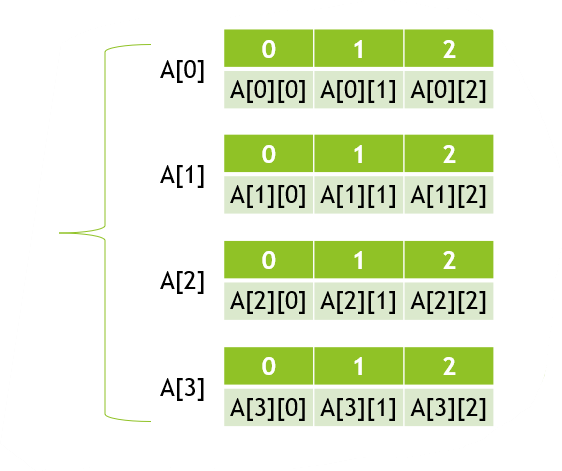
\includegraphics[width=0.5\textwidth]{2d_array.png}
    \caption{二維陣列圖解}
    \label{2d_array}
\end{figure}
那長度一、長度二具體是甚麼意思呢?我們可以看一下圖 \ref{2d_array},可以發現長度一的4可以想成二維陣列裡面放的一維陣列數量,也就是圖中的橫的那部分,而長度二則代表每個一維陣列的長度。

所以簡單來說,二維陣列可以想成在一個一維陣列再塞一維陣列。

\subsection{存取}
如圖 \ref{2d_array} 二維陣列的每個值就像是表格中所填的那樣,第一個方括號是用來選取是哪個一維陣列,第二個方括號是用來選取是一維陣列中的哪個值。

\subsection{初始化}
初始化主要有下面幾種寫法:
\begin{code}
    \captionof{listing}{二維陣列的初始化}
    \begin{minted}
#include <iostream>
using namespace std;
int main(){
    int A[4][3]; // 自動補0
    int B[4][3] = {1, 2, 3, 4, 5, 6, 7, 8, 9, 10, 11, 12}; 
    // 按照[0][0], [0][1]的順序依序填入
    int C[4][3] = {
        {1, 2, 3},
        {4, 5, 6},
        {7, 8, 9},
        {10, 11, 12},
    }; // 寫成許多一維陣列的形式
    int D[][3] = {
        {1, 2, 3},
        {4, 5, 6},
        {7, 8, 9},
        {10, 11, 12},
    }; // 可以自動算長度,不過最後一個長度一定要是給定的
}
\end{minted}
\end{code}
\section{多維陣列}
\begin{figure}[h]
    \centering
    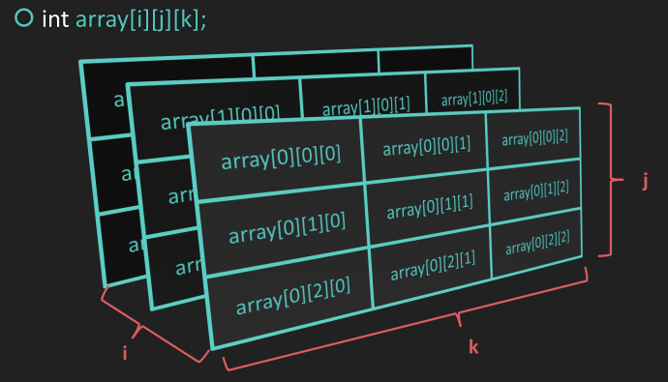
\includegraphics[width=0.7\textwidth]{3d_array.png}
    \caption{多維陣列?}
    \label{xd_array}
\end{figure}
除了二維陣列以外,我們可以在宣告時加上更多的方括號,成為多維陣列。

其實更高維度的陣列也可以用前面的思考方式,想成在陣列裡面塞陣列,像三維陣列就是把一個陣列塞一個陣列,那一個陣列裡面再塞一個陣列。

多維陣列的具體使用方法和二維陣列差不多,我就不再多講一次。

\textbf{小問題:\texttt{int A[i][j][k][l]}這個陣列裡面有幾個元素呢?}

\chapter{字元與字串}
\section{字元}
字元(char)代表的可以是一個數字、字母或是符號。在程式中,我們會以ASCII碼(\url{https://zh.wikipedia.org/wiki/ASCII})來表示字元。
除了0123456789、abcdABCD、\# *@!()外,還有一些控制字元(不會顯示在畫面上),像是:

\begin{table}[H]
    \centering
    \begin{tabular}{|c|c|}
        \hline
        控制字元                     & 說明            \\ \hline
        \texttt{'\textbackslash{}t'} & 定位字元(TAB)   \\ \hline
        \texttt{'\textbackslash{}n'} & 換行(ENTER)     \\ \hline
        \texttt{'\textbackslash{}r'} & 回車(RETURN)    \\ \hline
        \texttt{'\textbackslash{}b'} & 倒退(Backspace) \\ \hline
        \texttt{'\textbackslash{}0'} & 字串結尾        \\ \hline
    \end{tabular}
\end{table}

\begin{code}
    \captionof{listing}{字元宣告與初始化方式}
    \begin{minted}
#include <iostream>
using namespace std;
int main(){
    char A;//宣告一個字元
    char B = 97;//宣告字元並設初始值為97
    char C = 'a';
}
\end{minted}
\end{code}
在程式碼中,會以char型態儲存一個字元。若要表示一個字元,會以一對單引號(')將字元夾起來。在先前有提過,char型態存的是ASCII數值,所以'a'會對應到97,並將值賦給char。

如果想要表示單引號(')要怎麼辦呢?這時,就要在前面加上反斜線(\textbackslash)來表示,反斜線(\textbackslash)又稱為「跳脫字元(escape character)」,可以用來表示特殊字元,例如:
\begin{table}[H]
    \centering
    \begin{tabular}{|c|c|}
        \hline
        特殊字元                  & 表示方法                                  \\ \hline
        單引號(\texttt{'})        & \texttt{\textbackslash{}'}                \\ \hline
        雙引號(\texttt{"})        & \texttt{\textbackslash{}"}                \\ \hline
        \texttt{\textbackslash{}} & \texttt{\textbackslash{}\textbackslash{}} \\ \hline
        控制字元                  & 如先前所提                                \\ \hline
    \end{tabular}
\end{table}

由於字元本身就是一個整數,所以它可以做運算。以下的等號都是成立的:
\begin{code}
    \captionof{listing}{字元運算}
    \begin{minted}
'b' == 'a' + 1
'A' == 'a' ^ ' '
2 == 'c' - 'a'
'y' == ('c' + 'h' + 'a' + 'r')%26 + 'a'
\end{minted}
\end{code}
\section{字串}
字串(string),顧名思義就是把字元串在一起。
\begin{code}
    \captionof{listing}{字串(string)}
    \begin{minted}
#include <iostream>
#include <cstring> //for string
using namespace std;
int main(){
    char A[9];//宣告長度為9個字元的陣列
    string B;
    cin >> A >> B;
    cout << A[0] << B[0];
    cout << A << B;
}
\end{minted}
\end{code}
\subsection{宣告}
首先看到main function的第一行,字元陣列宣告方式為"char 字元陣列名稱[字串長度]"。此外,也可以引入<cstring>標頭檔,宣告方式為 ``string 字串名稱"。
\subsection{存取}
再來是第$3 \sim 5$行,先前兩種宣告方式都可以
\begin{enumerate}
    \item 讀入整行字串(第4行)。若用cin>>讀入,會讀到' ','\textbackslash{}t','\textbackslash{}n'為止。
    \item 存取字串中某個字元(第5行)。
    \item 存取整個字串(第6行)。在每個字串的最後,皆會有'\textbackslash0'作結。故輸出到'\textbackslash0'時,會停止輸出。
\end{enumerate}

\subsection{初始化}

\begin{code}
    \captionof{listing}{字串初始化}
    \begin{minted}
#include <iostream>
#include <cstring> //for string
using namespace std;
int main(){
    char A[] = {'s','t','r','i','n','g'};
    char B[] = "string";
    string C = "string";
    char D[6] = "string";//這是錯誤的初始化方式,可能會無法compile
}
\end{minted}
\end{code}
在初始化時,可以char型態的陣列一樣以char分開儲存。但這樣太麻煩了,所以我們可以用雙引號(")將字串夾起來。在main function中的第4行是錯誤的,為什麼呢?這是因為字串會以\texttt{'0'}結尾,所以若用字元陣列宣告的字串長度必須加1。

\subsection{文字處理函式}
\url{https://en.cppreference.com/w/cpp/string/byte}有詳細整理各種函式,以下整理常用函式。

獲取文字系列:
\begin{itemize}
    \item \texttt{cin.get()}:讀取下一個字元(包括空白字元' '、換行字元'\textbackslash{}n')
    \item \texttt{cin.get(陣列A, 讀取數量n)}:讀取n個字元至陣列A
    \item \texttt{cin.getline()}:讀取整行(包括空白字元' ')
    \item \texttt{getchar()}:讀取一個字元
\end{itemize}
str系列,以下函式必須加入\texttt{\#include<cstring>}才能使用:
\begin{itemize}
    \item \texttt{strlen(字串)}:得到字串長度
    \item \texttt{strcmp(字串A, 字串B)}:回傳0表示AB一樣,回傳1表示AB不一樣
    \item \texttt{strcpy(字串A, 字串B)}:把B複製到A
\end{itemize}
以下函式必須加入\texttt{\#include<cctype>}才能使用:

is**系列,如果字元屬於**則回傳1,否則回傳0:
\begin{itemize}
    \item \texttt{isalpha(字元)}:判斷字母
    \item \texttt{isdigit(字元)}:判斷數字
    \item \texttt{isspace(字元)}:判斷空白
\end{itemize}

to**系列,將字元轉成**:
\begin{itemize}
    \item \texttt{tolower(字元)}:轉成小寫
    \item \texttt{toupper(字元)}:轉成大寫
\end{itemize}
% \chapter{Struct}

\chapter[資料結構 Data Structure]{資料結構 Data Structure\footnote{此章參考建中資訊培訓講義}}

相信大家都是C或者C++的使用者。

如果你C的使用者,強烈建議你現在開始使用C++。語法相容,但又有強力的library,是你在競賽時間壓力下不可或缺的強力工具。

如果你是C++的使用者,強烈建議你把C++內建又好用的東西摸熟。這樣就可以省去許多功夫,開心使用前人為你寫好的東西了。

\section{什麼是資料結構}
就是字面上的意思:儲存資料的結構。

像前面有提到的陣列就是一種資料結構,它直接把一堆同樣型別的資料排成一排好好管理。但除了陣列之外,還有許多資料結構(有些甚至不是內建的)是需要瞭解的。以下就講些簡單常用的內建資料結構吧。

這些資料結構在「標準模板庫」(Standard Template Library,簡稱 STL)之中,是一個C++ 的程式庫。注意,這個程式庫的所有東西都在 \texttt{namespace std} 底下。

\section{型別模板 (Template)}

不過在繼續之前,有個重要的 C++ 觀念要講。

試想有一個作為容器用的型別 \texttt{C},可以容納一些型別是給定的型別 \texttt{T} 的東西。那你
在宣告這樣的一個變數時,理論上你應該告訴編譯器這個變數容納的型別是哪個型別。然而 C 語言中並沒有這樣的語法,所以在這樣的需求下模板(template)就在 C++ 誕生了。

型別模板的功用就是生出一堆新的型別。比方說剛剛的 \texttt{C} 好了,存放 \texttt{int} 型別的 \texttt{C} 和存放 \texttt{double} 型別的 \texttt{C},型別應該要是不同的。所以在宣告一個變數時,不是寫「\texttt{C (變數名)}」,而是寫「\texttt{C<(int 或 double)> (變數名)}」以指定這個變數的型別要是存放 int 的那種型別,還是存放 double 的那種型別。

有些型別模板的參數不只一個,寫好寫滿就對了(例:\texttt{priority\_queue<A, B, C>} 就需要三個型別)。如果沒有寫好寫滿,會自動採用預設的型別(前提是要有預設的)。

想瞭解更多的話,關鍵字搜「模板」跟「C++」吧。

註:C++11 開始,模板的參數數是可變的。

\section{迭代器 (Iterator)}

設想有個容器 \texttt{C},裡面已經裝一些東西了。我該如何遍歷 \texttt{C} 中的所有元素呢?要知道 C 可能長得不像陣列,沒有「下標」這種東西。為了解決這個問題,C++ STL 為每個容器提供一個成員型別,叫做「迭代器」。

你可以把迭代器想像成是指標(事實上,指標也算一種迭代器)。如果你今天有一個迭代器 \texttt{i},存取 \texttt{i} 指向的內容的方法,跟指標一樣,是在前面加個星號(\texttt{*i})。而迭代器分成三種,取決於迭代器能進行的運算,由功能強到弱排序如下:
\begin{enumerate}
    \item 隨機存取 (Random Access) 迭代器:這這類迭代器能夠和整數做加減法,加 s 代表從這項開始往後數 s 項,減 s 代表往前數 s 項。當然,遞增、遞減運算也沒有問題。你可以把指標當作這種迭代器。

    \item 雙向 (Bidirectional) 迭代器:這類的迭代器只能做遞增(\texttt{++})和遞減(\texttt{--})運算,分別代表後一項和前一項。
    \item 單向 (Forward) 迭代器:這類的迭代器只能做遞增(\texttt{++}),代表後一項。
\end{enumerate}

而按照迭代器的使用方法,分成兩種:
\begin{enumerate}
    \item 輸入 (Input) 迭代器:當你只有要讀取迭代器指向的內容時,這時迭代器當作輸入迭代器使用。所有的迭代器都可以當作輸入迭代器。
    \item 輸出(Output)迭代器:當你要直接更改迭代器指向的內容時,這時迭代器當作輸出迭代器使用。除了常數(const)迭代器(也就是規定不能更動迭代器指向的內容)以外, 所有的迭代器都可以當作輸出迭代器。
\end{enumerate}

C++ 內建的迭代器都很和藹,只要是可以做的運算,複雜度都是 O(1)。

為了滿足人們的需求,C++ 內建的容器通常有兩種迭代器:正常的迭代器以及逆向迭代器。假如容器的型別是 \texttt{C},因為迭代器是原本型別的成員型別,宣告時名稱分別是\texttt{C::iterator} 和 \texttt{C::reverse\_iterator}。前者會從前迭代到後,後者會從後迭代到前。另外,每個容器 \texttt{c} 的兩種迭代器各有兩個迭代器代表頭尾,分別是\texttt{c.begin()、c.end()} 和 \texttt{c.rbegin、c.rend()}。\texttt{c.begin()} 指向 \texttt{c} 的第一項,而 \texttt{c.end()} 指向 \texttt{c} 的最後一項的\textbf{後一項}。也就是說,\texttt{*c.end()、*c.rend()} 是不存在的,如果你這樣寫會造成不可預期的後果。

\section{vector}

vector位於標頭檔 \texttt{<vector>}中,vector可以視為動態陣列的實現。一般的陣列在宣告時就確定了,然而vector的長度可以任意伸縮。

以下vector的常用語法 (假設變數名為 \texttt{v}):

\begin{enumerate}
    \item (建構式) \texttt{vector<T> v(size\_type a, const T\& b)}:一開始這個\texttt{v}會被 \texttt{b}填滿,總共填 \texttt{a} 個。如果只有指定\texttt{a},那麼\texttt{b}會是\texttt{T}的預設值。如果\texttt{a, b}都沒有指定,那\texttt{v}會是一個空的vector。建構複雜度$O(a)$。
    \item \texttt{v[i]}:\texttt{v}中第 \texttt{i} 項,就把這個語法想成陣列就好。複雜度$O(1)$。
    \item \texttt{v.size()}:這個函式會回傳 \texttt{v} 目前的長度。複雜度$O(1)$。
    \item \texttt{v.push\_back(T a)}:在 \texttt{v} 的尾端加一個 \texttt{a}。均攤複雜度$O(1)$。
    \item \texttt{v.pop\_back()}:刪除 \texttt{v} 的最末項。如果\texttt{v}是空的,會發生不可預期的結果。複雜度$O(1)$。
    \item \texttt{v.clear()}:清空 \texttt{v}。複雜度 $O(size)$。原本 \texttt{v} 的空間會被保留,不會釋放掉。
    \item \texttt{v.resize(size\_type a, const T\& b)}:強制將 \texttt{v} 的長度變為 \texttt{a}。如果比原本短,則將 \texttt{v} 原本的末段捨去,複雜度 $O(D(size − a))$,$D$ 是解構 \texttt{T} 的時間。如果比原本長,在 \texttt{v} 的後面加 \texttt{b} 直到足夠為止(如果只有指定 \texttt{a},那麼 \texttt{b} 是 \texttt{T} 的預設值),通常複雜度$O(C(a − size))$,但如果需重新配置記憶體(reallocate),複雜度 $O(Ca)$,其中 $C$ 是建構(複製)\texttt{T} 的時間。
    \item \texttt{v.reserve(size\_type n)}:預留放至少 $n$ 個 \texttt{T} 的空間。如果需重新配置記憶體,複雜度$O(size)$。如果 $n < size$,這個函數不造成任何影響。
\end{enumerate}

vector 的迭代器屬於隨機存取(Random Access)迭代器。

比較需要講的是 vector 重新配置記憶體的耗時較長,所以如果能預先知道記憶體最多
需要多少,就在一開始建構的時候開滿或者先 \texttt{reserve} 吧!(儘管對時間只有常數的影響)

另外,\texttt{vector<bool>} 有神奇優化成一個 bool 佔的空間只有 1 bit,是 \texttt{bool[]} 的 1/8。

\section{string}

string 位於標頭檔\texttt{<string>} 裡,等價於 \texttt{basic\_string<char>}(如果不知道這個,可能會
看不懂編譯訊息)。string 的用法很像 \texttt{vector<char>},但因字串太常使用了,所以有經過一些優化。除此之外,還有一些好用的東西(假設變數名為 \texttt{s}):

\begin{enumerate}
    \item \texttt{s = t}:如果 \texttt{t} 是一個 string 或是 C 式字串,\texttt{s} 會變得跟 \texttt{t} 一樣。複雜度不明,但通常是$O(size_s + size_t)$。
    \item \texttt{s += t}:如果 \texttt{t} 是一個 string 或是 C 式字串,在 \texttt{s} 的尾端加上 \texttt{t}。複雜度通常是 $O(size_s+size_t)$。
    \item \texttt{s.c\_str()}:這個函式會回傳跟 \texttt{s} 一樣的 C 式字串。在 C++11 中保證複雜度為 $O(1)$。
    \item \texttt{s }(比較大小或相等的符號)\texttt{ t}:回傳比較 \texttt{s} 跟 \texttt{t} 字典序的結果。通常複雜度是$O(max(size_s, size_t))$。
    \item \texttt{cin >> s}:輸入字串至\texttt{s},直到讀到空白字元。
    \item \texttt{cout << s}:輸出字串 \texttt{s}。
          \item\texttt{getline(cin, s, char c)}:輸入字串至 \texttt{s},直到讀到字元 \texttt{c}。未指定時,\texttt{c} 是換行符號(\texttt{'\textbackslash n'})。
\end{enumerate}

string 的迭代器屬於隨機存取迭代器。

除了列舉的之外,vector 有的 string 都有。除此之外,s.size() 有個同義的函式\texttt{s.length()},可能是怕人打錯才多加了這個函式吧。

順帶一提,關於 string 是不是「容器」其實也有些爭議,但它有大部分容器的性質,所以在此仍然將其歸類為容器。

\section{deque}

deque 位於標頭檔 \texttt{<deque>} 裡。deque 可以視為可以在最前面加東西、刪東西的vector,除此之外它就是 vector 了。

假設變數名是 \texttt{d},想要移除第一項,就用 \texttt{d.pop\_front()}。想要在前面加一個東西 \texttt{a},就用 \texttt{d.push\_front(a)}。這兩個函式不會使迭代器失效,但會改變 deque 的下標。

雖說功能比 vector 強,但代價是時間和空間幾乎翻倍,所以沒事別用 deque。

\section{list}
list 位於標頭檔 \texttt{<list>} 裡。list 是個「雙向鏈結(doubly linked)結構」,也就是說對於
list 中的每一項,都可以 $O(1)$ 知道它的前一項和後一項。如此做的好處是,如果我要一次性加入一堆東西,只需要 $O(1)$ 的代價,比 vector 優。然而代價是,存取第 $i$ 項的複雜度是$ O(i)$,因此沒有內建的下標運算。同樣列舉一下常用語法(假設變數名為 \texttt{s}):

\begin{enumerate}
    \item (建構式)\texttt{list<T> s(size\_type a, const T\& b)}:同 vector。
    \item \texttt{s.push\_front(T a)、s.push\_back(T a)、s.pop\_front()、s.pop\_back()}:同 deque。
    \item \texttt{s.size()}:回傳 \texttt{s} 中有幾項。相當需要注意的是 C++98 中這個函式的複雜度只有保證$O(size)$,C++11 則保證 $O(1)$。
    \item \texttt{s.empty()}:回傳一個 bool,代表 \texttt{v} 是否是空的。複雜度 $O(1)$。
    \item \texttt{s.insert(iterator p, T a)}:在 \texttt{p} 指的那一項前面插入一個 \texttt{a} 並回傳一個指向 \texttt{a} 的迭代器。複雜度$O(1)$。
    \item \texttt{s.insert(iterator p, size\_type n, T a)}:在 \texttt{p} 指的那一項前面插入 \texttt{n} 個 \texttt{a}。複雜度 $O(n)$。
    \item \texttt{s.erase(iterator p)}:把 \texttt{p} 指的那項刪掉並回傳指向之後那項的迭代器。注意刪完之後 \texttt{p} 就失效了。複雜度 $O(1)$。
    \item \texttt{s.erase(iterator first, iterator last)}:把 [first,last) 指到的東西全砍光光,回傳 \texttt{last}。複雜度和砍掉的東西個數呈線性關係。
    \item \texttt{s.splice(iterator p, list\& x, iterator first, iterator last)}:\texttt{first} 和 \texttt{last} 是 \texttt{x} 的迭代器。這個函式會把 [\texttt{first},\texttt{last}) 指到的東西從 x 中移除並加到 p 指的那項前面。注意到 \texttt{x} 會因為這個函式而改變。如果沒有指定 \texttt{last},那只將 \texttt{first} 從 \texttt{x} 刪去並加入 \texttt{s}。如果 \texttt{first} 和 \texttt{last} 都沒指定,那會將 \texttt{x} 中所有東西移到 \texttt{s} 中使 \texttt{x} 變為空的。複雜度是轉移元素個數的線性。
\end{enumerate}

list 的迭代器屬於雙向迭代器。

可以看出 list 最大的功能是可以用 $O(1)$ 的代價進行一些別的容器做不到的事(\texttt{insert}、\texttt{erase})。然而 list 最大的問題是所佔空間過於龐大,而且實用性低。C++11 中多了一個 forward\_list 以改善空間過大的問題,代價是迭代器變成單向迭代器(也因此沒有\texttt{reverse\_iterator})。

\section{stack}

stack 位於標頭檔 \texttt{<stack>} 裡。可以把它想像成一疊書,每次可以放一本書在最上面,也可以從最上面拿一本書走。簡單來說就是秉持著「後進先出」(LIFO)的精神。

stack 這個模板需要的型別參數有兩個:\texttt{T} 和 \texttt{C},其中 \texttt{T} 是內容物的型別,而 \texttt{C} 是採用的容器。為了方便改造,stack 對 C 有些要求:要有 \texttt{empty、size、back、push\_back、pop\_back} 這些函式,而在內建的容器中能夠勝任這角色的有 vector、deque 和 list。

stack 常用的語法列舉如下(假設變數名為 \texttt{s}):

1.(建構式)\texttt{stack<T, C> s(C\& a)}:\texttt{s} 一開始會有一份 \texttt{a} 的複製品。如果沒有指定 \texttt{C} 的話,\texttt{C}是\texttt{deque<T>}。如果沒有指定 \texttt{a} 的話,\texttt{s} 一開始會是空的。複雜度 $O(size)$。
2. \texttt{s.size()、s.empty()}:同 vector。
3. \texttt{s.top()}:存取最後一個進入 \texttt{s} 的元素,即「一疊書中最上面的那一本」。複雜度 $O(1)$。
4. \texttt{s.push()}:將一個元素加入 s 中。複雜度 $O(1)$。
5. \texttt{s.pop()}:將最後一個進入 s 的元素移除。複雜度 $O(1)$。

至於 \texttt{C} 應該要選用什麼,個人建議是 \texttt{vector<T>}。而且事實上,stack 能做的事 vector都能做到,所以平常用 vector 就可以了。只是用 stack 可以增加程式的可讀性。


\section{queue}

queue 位於標頭檔 \texttt{<queue>} 裡。可以把它想像成排隊等著結帳的人群,要嘛有新的人來排在隊伍的尾端,要嘛最前面有一個人結完帳要走了。簡單來說,就是秉持著「先進先出」(First In, First Out; FIFO)的精神。

queue 這個模板同樣需要兩個型別參數 \texttt{T} 和 \texttt{C},跟 stack 一樣。不過不同的是,queue對 C 的要求不太一樣:要有 empty、size、front、back、push\_back、pop\_front 這些函式,而在內建的容器中能夠勝任這角色的只有 deque 和 list。

queue 常用的語法列舉如下(假設變數名為 \texttt{q}):

\begin{enumerate}
    \item (建構式)\texttt{queue<T, C> q(C\& a)}:q 一開始會有一份 \texttt{a} 的複製品。如果沒有指定 \texttt{C} 的話,\texttt{C} 是 \texttt{deque<T>}。如果沒有指定 \texttt{a} 的話,\texttt{q} 一開始會是空的。複雜度 $O(size)$。
    \item \texttt{q.size(),q.empty()}:同 vector。
    \item \texttt{q.front()}:存取第一個進入 \texttt{q} 的元素,即「隊伍中最前面的人」。複雜度 $O(1)$。
    \item \texttt{q.back()}:存取最後一個進入 \texttt{q} 的元素,即「隊伍最末端」。複雜度 $O(1)$。
    \item \texttt{q.push()}:將一個元素加入 \texttt{q} 中。複雜度 $O(1)$。
    \item \texttt{q.pop()}:將第一個進入 \texttt{q} 的元素移除。複雜度 $O(1)$。
\end{enumerate}

建議 \texttt{C} 就依照預設的即可。不過和 stack 一樣,要用 queue 不如用 deque。
\section{priority\_queue}

\texttt{<queue> }中其實還藏有一威力極大的適配器:priority\_queue。priority\_queue 利用幾個內建函式實現「二叉堆」(binary heap)結構,一個在任何時候維持最頂的元素永遠都是最大的資料結構。priority\_queue 雖然實作容易,但應用廣泛,每次都手刻一次會很浪費時間。以後會見到更多 priority\_queue 的應用。

priority\_queue 這個模板需要三個型別參數 \texttt{T、Con 和 Cmp}。\texttt{T} 代表內容物的型別(需可以比較大小),\texttt{Con} 代表使用的容器,而 \texttt{Cmp} 代表使用的比大小的依據(之後會再詳細說明)。Con 的要求是擁有隨機存取迭代器以及 \texttt{empty、size、front、push\_back、pop\_back}這些函式,而滿足這些條件的內建函式有 vector(預設值)和deque。在詳細地認識 \texttt{Cmp}之前,只需要知道 \texttt{Cmp} 是 \texttt{less<T>}(預設值)時 \texttt{priority\_queue} 是最大堆,而是 \texttt{greater<T>}的時候 \texttt{priority\_queue} 是最小堆。

priority\_queue 常用的語法列舉如下(假設變數名為 \texttt{pq}):

\begin{enumerate}
    \item (建構式)\texttt{priority\_queue<T, Con, Cmp> pq}:建構一個空的 \texttt{pq}。複雜度 $O(1)$。
    \item (建構式)\texttt{priority\_queue<T, Con, Cmp> pq(iterator first, iterator last)}:建構一個 pq,內含\texttt{[first,last)} 指到的東西,這裡 iterator 可以是任何迭代器。複雜度$O(size)$。
    \item \texttt{pq.size()、pq.empty()}:同 vector。
    \item \texttt{pq.top()}:回傳 \texttt{pq} 中最大(最小)的元素(無法修改)。複雜度 $O(1)$。
    \item \texttt{pq.push(T a)}:將 \texttt{a} 加入 \texttt{pq} 中。複雜度 $O(\log size)$。
    \item \texttt{pq.pop()}:將 \texttt{pq} 中最大(最小)的元素移除。複雜度 $O(\log size)$。
\end{enumerate}

比較需要注意的是在建構的時候直接餵內容物的時間複雜度是 $O(size)$,而一個一個push進去的時間複雜度是 $O(size \log size)$。雖然一般情況下沒什麼差,不過有必要的時候請記得 priority\_queue 的建構式可以減少複雜度。

\section{pair}

pair 位於標頭檔\texttt{<utility>}裡面(注意沒有 <pair> 這個標頭檔)。pair 其實很單純,就是把兩個(可能不同型別的)變數綁在一起,變成一個變數。為此,pair 需要接收兩個型別,分別代表一對的第一項和第二項的型別。

pair 常用的語法列舉如下(假設變數名為 \texttt{p}):

\begin{enumerate}
    \item (建構式)\texttt{pair<A, B> p(A a, B b)}:建構一個把型別 \texttt{A} 和型別 \texttt{B} 綁在一起的 \texttt{p},其中第一項是 \texttt{a},第二項是 \texttt{b}。
    \item \texttt{p = s}:如果 \texttt{s} 也是同型別的 pair,把 \texttt{p} 變得跟 \texttt{s} 一樣。
    \item \texttt{p}(比較大小或相等的符號)\texttt{s}:如果 \texttt{s} 也是同型別的 pair,先比第一項,如果一樣再比第二項。
    \item \texttt{p.first、p.second}:存取第一項、第二項。
\end{enumerate}

在使用 pair 時,常常會使用到一個非成員函式 \texttt{make\_pair}。\texttt{make\_pair} 的好處在於,你不用特別指明第一項和第二項的型別,編譯器會自行幫你解析。用法是 \texttt{make\_pair(A a,B b)},函式會回傳一個 \texttt{pair<A, B>},其中第一項是 \texttt{a},第二項是 \texttt{b}。

另外,C++11 開始允許可變長度的模板,所以也有 pair 的推廣版 tuple(在標頭檔\texttt{<tuple>} 中)。有興趣的可以自己看看。

\section{set}

set 位於標頭檔 \texttt{<set>} 裡。set 實現了自平衡二元查找樹,用白話文來講,可以 $O(\log n)$插入、刪除或查詢一個值有沒有在其中。特別的是,裡面的元素不會重複,因此我們會把元素的值稱為鍵值(key)。

set 的常用語法列舉如下(假設變數名為 \texttt{s}):
\begin{enumerate}
    \item (建構式)\texttt{set<K> s}:建構一個空的 \texttt{s}。複雜度 $O(1)$。
    \item \texttt{s.size()、s.empty()}:同 vector。
    \item \texttt{s.insert(K k)}:在 \texttt{s} 中放入一個鍵值為 \texttt{k} 的元素。如果本來就有了,什麼事都不會做。複雜度 $O(\log size)$。
    \item \texttt{s.erase(iterator first, iterator last)}:刪除 \texttt{[first,last)}。如果沒指定 \texttt{last},只刪除 \texttt{first}。只刪除一個時,均攤複雜度 $O(1)$,刪除多個時複雜度是刪除個數的線性。
    \item \texttt{s.erase(K k)}:刪除所有鍵值為 \texttt{k} 的元素並回傳刪除的項數(在 set 中只會是 0 或 1)。複雜度$O(\log size)$。
    \item \texttt{s.find(K k)}:回傳指向鍵值為 \texttt{k} 的元素的迭代器。如果沒有這種東西,回傳 \texttt{m.end()}。複雜度 $O(\log size)$。
    \item \texttt{s.count(K k)}:回傳有幾個鍵值為 \texttt{k} 的元素(在 set 中只會是 0 或 1)。複雜度 $O(\log size)$。
    \item \texttt{s.lower\_bound(K k)}:回傳迭代器指向第一個鍵值大於等於 \texttt{k} 的項。複雜度 $O(\log size)$。
    \item \texttt{s.upper\_bound(K k)}:回傳迭代器指向第一個鍵值大於 \texttt{k} 的項。複雜度 $O(\log size)$。
\end{enumerate}

set 的迭代器是雙向迭代器。\texttt{set::iterator} 會由小迭代到大,\texttt{set::reverse\_iterator} 則會由大迭代到小。比較容易被忽視的是 set 的迭代器在遞增和遞減的時候,理論上不只是均攤複雜度,連複雜度也是 $O(1)$。但有些實作只保證均攤複雜度。

要注意的是 \texttt{lower\_bound} 和 \texttt{upper\_bound} 的微妙差別:一個是大於等於、一個是大於。用途通常是找鍵值在 \texttt{[l,u)} 的那些項,找法是 \texttt{[s.lower\_bound(l), s.upper\_bound(u))}。記住,C++ 通常是左閉右開區間。

\section{map}
map 位於標頭檔 \texttt{<map>} 裡。map 可以當成 set 的每一個元素都對應到另一個值,也就是可以用 $O(\log n)$ 插入、刪除或尋找一個鍵值對應的值。因此,map 這個模板需要兩個型別參數 \texttt{K} 和 \texttt{T},其中 \texttt{K} 是鍵值的型別(需要可以比大小),而 \texttt{T} 代表對應到的值的型別。

另外,map 中的每一個元素其實是 \texttt{pair<K, T>},所以迭代器指向的東西是一個 pair,第一項是鍵值,第二項是對應的值。

map 常用的語法列舉如下(假設變數名為 \texttt{m}):

\begin{enumerate}
    \item (建構式)\texttt{map<K, T> m}:建構一個空的 \texttt{m}。複雜度 $O(1)$。
    \item \texttt{m.size()、m.empty()、m.erase(iterator first, iterator last)}\\\texttt{、m.erase(K k)、m.find(K k)、m.count(K k)、m.lower\_bound(K k)、m.upper\_bound(K k)}:同 set。
    \item \texttt{m[k]}:存取鍵值 \texttt{k} 對應的值。如果 \texttt{k} 沒有對應的值,會插入一個元素,使 \texttt{k} 對應到預設值並回傳之。複雜度 $O(\log size)$。
    \item \texttt{m.insert(pair<K, T> k)}:如果沒有鍵值為 \texttt{k.first} 的值,插入一個鍵值為 \texttt{k.first} 的值對應到 \texttt{k.second},並回傳一個 pair,\texttt{first} 是指向剛插入的元素的迭代器、\texttt{second} 是 true;如果已經有了,回傳一個 pair,\texttt{first} 是指向鍵值為 \texttt{k.first} 的元素的迭代器,\texttt{second} 是false。複雜度 $O(\log size)$。
\end{enumerate}

和 set 的迭代器一樣,map 的迭代器是雙向迭代器。

\section{multiset, multimap}

在 \texttt{<set>、<map>} 中分別還有 multiset 和 multimap。和前面大致相同,唯一的差別在於 multiset 和 multimap 中鍵值可以重複出現,不像 set 和 map 鍵值不能一樣。如此一來,\texttt{count} 和 \texttt{erase} 回傳的值便不一定是 0 或 1。此外,由於 multimap 中一個鍵值可能對應到許多不同的值,因此也不支援下標操作。

在 multiset 和 multimap 中有一個特別好用的函式 \texttt{equal\_range(K k)},會回傳一個 iterator的 pair,第一項代表\texttt{lower\_bound(k)},第二項代表 \texttt{upper\_bound(k)}。這兩項迭代器之間的項就是那些鍵值是 \texttt{k} 的項。雖然這個函式 set 跟 map 也有,但在 set 和 map 中就顯得有點雞肋。

\section{(C++11)unordered\_(multi)set, unordered\_(multi)map}
在 C++11 以後,unordered 系列常常擔任優化掉 map 和 set $O(\log n)$ 複雜度的角色。

unordered\_(multi)set 和 unordered\_(multi)map 分別在標頭檔 \texttt{<unordered\_set> 和 <unordered\_map>} 裡。這四個模板需要的前一(二)個型別參數和 set(map)一樣,而接著是一個型別Hash,代表要使用的雜湊函數的函數型別(之後會提)或指標。不過 C++11 有預設的內建型別(含任意型別的指標)的雜湊函數,所以除非情況特殊,你可以不用理會這一項。

你可以把 unordered 系列當成 (multi)map 和 (multi)set 來用。不過有幾點不同:
\begin{enumerate}
    \item unordered 系列的迭代器為單向迭代器。
    \item unordered 系列沒有將所有項依鍵值排序(這也是它名字的由來),因此迭代器在遍歷容器時不會依鍵值的大小順序遍歷。
    \item 因為沒有排序,所以理所當然的沒有 lower\_bound、upper\_bound。
    \item 比起 (multi)map 和 (multi)set,unordered 系列的期望複雜度少一個 $\log$。
\end{enumerate}

在宣告變數(建構式)時,你可以指定 bucket 至少有幾個。如果鍵值是內建型別而且你沒有指定 bucket 至少有幾個,那麼它會很耐斯地幫你搞定。

\section{bitset}

bitset 位於標頭檔 \texttt{<bitset>} 裡。你可以把它想像成有一堆 0 跟 1 的一個陣列,也就是說 bitset 的大小是固定的。但是它每一項只會用到 1 bit 的空間,而 bitset 的位元運算是被優化過的(雖然只限於同大小的 bitset),運作起來非常快速,對常數有極巨大的影響,同時也可以達到壓縮空間的效用,是常數優化的好幫手。

bitset 這個模板需要一個整數 \texttt{n} 作為模板的參數,代表 bitset 的長度。

bitset 的一些常用語法列舉如下(假設變數名為 \texttt{b}):
\begin{enumerate}
    \item (建構式)\texttt{bitset<N> b(a)}:用 \texttt{a} 初始化一個長度為 \texttt{N} 的 bitset。這裡 \texttt{a} 可以是 unsigned long、string 或 C 式字串。如果沒有指定 \texttt{a},或者如果 \texttt{b} 有一些地方沒被 \texttt{a} 初始化,那些地方預設為 0。
    \item \texttt{b.count()}:回傳 \texttt{b} 有幾個位元是 1。複雜度 $O(N)$。
    \item \texttt{b.size()}:回傳 \texttt{b} 有幾個位元。複雜度 $O(1)$。
    \item \texttt{b (位元運算)}:不管是一元還是二元的位元運算都可以。如果是兩個 bitset 的二元位元運算,兩個 bitset 的長度需一致。複雜度 $O(N)$。
    \item \texttt{b[a]}:存取第 \texttt{a} 位。複雜度 $O(1)$。
    \item \texttt{b.set()}:將所有位元設為 1。複雜度 $O(N)$。
    \item \texttt{b.reset()}:將所有位元設為 0。複雜度 $O(N)$。
    \item \texttt{b.flip()}:將所有位元的 0、1 互換(反白)。複雜度 $O(N)$。
    \item \texttt{b.to\_string()}:回傳一個字串和 \texttt{b} 的內容一樣。複雜度 $O(N)$。
    \item \texttt{b.to\_ulong()}:回傳一個 unsigned long 和 \texttt{b} 的內容一樣(在沒有溢位的範圍內)。複雜度$O(N)$。
\end{enumerate}

bitset 不是容器,而且它也沒有迭代器。

通常而言,如果要估計常數的話,相較於直接使用陣列,空間是 1/8、count 約是 1/6、位元運算約是 1/30。當然這些都不是絕對的。

要注意的是,上述的複雜度沒有明文規定,不過通常是如此。

\chapter{亂數 Random Number}
在寫程式時候,我們有時候會需要生成一定範圍內的亂數來完成某些任務。例如:寫一個抽籤程式、模擬擲骰子的過程、寫一個換位子的程式等等。亂數甚至還可以用來估算圓周率和解線性規劃問題等等。

在本章中,我們會講到要如何在程式中引入亂數。
\section{亂數的用法}
\begin{code}
    \captionof{listing}{亂數的用法}
    \label{code:rand}
    \begin{minted}
#include <iostream>
#include <cstdlib>
using namespace std;
int main(){
    for(int i=0; i<10; i++)
      cout << rand() % 1000 << endl;
}
\end{minted}
\end{code}
大家可以在電腦上執行看看\autoref{code:rand}~。可能會發現每次的執行結果都相同。這顯然不是我們想要的,因為這樣就不是亂數了嗎。

所以要怎麼辦呢?我們可以看看\autoref{code:randseed}
\begin{code}
    \captionof{listing}{srand()}
    \label{code:randseed}
    \begin{minted}
#include <iostream>
#include <cstdlib>
using namespace std;
int main(){
    srand(7122); // 設定亂數種子為 7122
    for(int i=0; i<10; i++)
        cout << rand() % 1000 << endl;
}
\end{minted}
\end{code}
Hmmm, 雖然輸出的數字不一樣了,但是每次執行所輸出的數字都一樣呀。所以到底要怎麼辦呢?
\begin{code}
    \captionof{listing}{srand(time(NULL))}
    \label{code:randtime}
    \begin{minted}
#include <iostream>
#include <cstdlib>
#include <ctime>
using namespace std;
int main(){
    srand(time(NULL)); // 設定亂數種子為程式執行當下的時間
    for(int i=0; i<10; i++)
        cout << rand() % 1000 << endl;
}
\end{minted}
\end{code}
可以發現在\autoref{code:randtime}~中, 我們將亂數的種子設成當下的時間,這樣每次執行時,亂數的種子都不會一樣,隨機出來的數字也都不一樣。我們的目的也就暫時完成了。

但其實以上的用法是最簡單的作法,隨機出來的數字不會是完美的隨機。如果想要了解更好的隨機方法,可以看看\href{https://reurl.cc/gmoNe4}{\underline{C++11 random}}。

\section{原理?}
\begin{code}
    \captionof{listing}{rand(), srand()的原始碼}
    \label{code:randsrc}
    \begin{minted}
static unsigned long int next = 1;

int rand(void) // RAND_MAX assumed to be 32767
{
  next = next * 1103515245 + 12345;
  return (unsigned int)(next/65536) % 32768;
}

void srand(unsigned int seed)
{
  next = seed;
}
\end{minted}
\end{code}
在\autoref{code:randsrc}~中,我們可以發現\texttt{rand()}是透過固定的運算產生下一個數字,而且亂數會有一個最大值\texttt{RAND\_MAX}。以這種方式產生的亂數稱為偽隨機亂數,但是一般來說,\texttt{rand()}函數對於一般的任務已經足夠了。

\chapter{二分搜尋 Binary Search}
在一群資料中搜尋某個資料,通常有\textbf{線性搜尋}和\textbf{二分搜尋}兩種。線性搜尋就是利用迴圈,從頭到尾的搜尋某個資料。對於沒有排序過的資料,線性搜尋是唯一的方法。但如果資料已經按照大小順序排列好了,我們就可以使用二分搜尋。使用二分搜尋($O(\log N)$)的效率相較於線性搜尋($O(N)$)好太多了。

在本章中,我們會提到要如何要怎麼寫基本的二分搜,也會介紹C++內建的二分搜函數及相關的資料結構。

\section{基本的二分搜}
最簡單的二分搜是在一個\textbf{排好序的陣列}中尋找某個元素,找到了回傳 index,否則回傳找不到(例如-1),這樣的二分搜好寫也不容易寫錯,以下是個範例。二分搜的重點在於 \texttt{left} 與 \texttt{right} 兩變數紀錄著搜尋範圍的左右邊界,每次取出中間位置來比較,結果是找到了或捨棄左半邊或捨棄右半邊。當 \texttt{left>right} 表示搜尋區間已經沒有了,這時離開迴圈,因為要找的元素不存在。若初始的區間範圍是 $N$,時間複雜度是 $O(\log N)$,原因是區間長度每次都減半。

\begin{code}
    \captionof{listing}{基本的二分搜}
    \label{code:binsea}
    \begin{minted}
#include <iostream>
using namespace std;
#define N 10
// binary search x between a[left..right]
int bsearch(int a[], int left, int right, int x) {
  while (left <= right) {
    int mid = (left + right) / 2;  // middle element
    if (a[mid] == x) return mid;
    if (a[mid] < x)
      left = mid + 1;  // search right part
    else
      right = mid - 1;  // search left part
  }
  return -1;
}
int main() {
  int p[N];
  int n = 10;
  for (int i = 0; i < n; i++) p[i] = rand() % 100;
  sort(p, p + n);
  for (int i = 0; i < n; i++) cout << p[i] << " ";
  cout << endl;
  printf("search %d => return %d\n", p[7], bsearch(p, 0, n - 1, p[7]));
  int t = rand() % 100;
  printf("search %d => return %d\n", t, bsearch(p, 0, n - 1, t));
  return 0;
}
\end{minted}
\end{code}

\section{C++的二分搜函數以及相關資料結構}
其實在C++中,提供了很多跟搜尋有關的函數和資料結構。這裡會介紹一些基本的用法。常用的二分搜函數有以下三種:
\begin{itemize}
    \item \texttt{binary\_search()}
    \item \texttt{lower\_bound()}
    \item \texttt{upper\_bound()}
\end{itemize}
\texttt{lower\_bound()}函數是用來找出第一個大於等於某個值的位置,而\texttt{upper\_bound()}是用來找出第一個大於某個值的位置,\texttt{binary\_search()}只回傳是否有這個值。

和\texttt{sort()}函數相同,\texttt{lower\_bound()}允許傳入自定義的比較函數。基本上呼叫的時候以\texttt{lower\_bound(first, last, t);},就可以搜尋在\texttt{[first, last)}範圍中,以二分搜搜尋第一個大於等於t的元素的位置。如果找不到時,就回傳\texttt{last}。

在使用\texttt{lower\_bound()}函數時,有幾點需要注意:
\begin{itemize}
    \item 找到元素時,回傳的是那個元素的\textbf{位置},如果想要得到索引值,還要再減去陣列的起始位置。
    \item 呼叫\texttt{lower\_bound()}函數時,必須確定搜尋範圍是排好序的,如果你針對一個未排序的資料以\texttt{lower\_bound()}進行二分搜,只會得到錯誤的結果。編譯器是不會告訴你資料沒有排序的。
    \item 搜尋範圍是傳統的左閉右開區間,也就是不含 \texttt{last}。
    \item 找不到時回傳 \texttt{last},通常這個位置是超過陣列的範圍,所以沒確定找到時不可以直接去引用該位置的值。
\end{itemize}

\autoref{code:lower}~是\texttt{lower\_bound()}函數的範例程式,執行一下就可以了\texttt{lower\_bound()}函數是在幹嘛的。
\begin{code}
    \captionof{listing}{\texttt{lower\_bound()}的使用方法}
    \label{code:lower}
    \begin{minted}
// demo lower_bound for int array
// binary search the first >=x
#include <bits/stdc++.h>
using namespace std;
#define N 5
int main() {
  int p[N] = {5, 1, 8, 3, 9};
  int n = 5;
  sort(p, p + n);
  for (int i = 0; i < n; i++) cout << p[i] << " ";
  cout << endl;
  for (int i = 0; i < 5; i++) {
    int t = i * 3;
    // search [first=p, last=p+n) to find the first >=t
    int ndx = lower_bound(p, p + n, t) - p;
    if (ndx < n)
      printf("The first >=%d is at [%d]\n", t, ndx);
    else  // return the last address if not found
      printf("No one >=%d\n", t);
  }
  // for vector
  vector<int> v(p, p + n);  // copy p to vector v
  for (int i = 0; i < 5; i++) {
    int t = i * 3;
    int ndx = lower_bound(v.begin(), v.end(), t) - v.begin();
    if (ndx < n)
      printf("The first >=%d is at [%d]\n", t, ndx);
    else  // return v.end() if not found
      printf("No one >=%d\n", t);
  }
  return 0;
}
\end{minted}
\end{code}
\chapter[動態規劃 Dynamic Programming]{動態規劃 Dynamic Programming\footnote{本章內容多參考吳邦一教授的\href{https://reurl.cc/q8bQVD
      }{\underline{《從 APCS 實作題檢測三級到五級》}}一書}}
這一章介紹動態規劃(Dynamic Programming, DP)。DP 名字中 Programming 的意思是指「以表格紀錄」,而非現在常用的「寫程式」,所以 DP 的意思是以變動的表格來求解的方法。DP的應用很廣,變化很多,在學術界也發展的很早,在程式競賽也用的非常多,並且有很多困難而精妙的(優化)方法。
\section{基本原理}
\subsection{基本思維與步驟}
DP與我們以後會提到的分治(Divide and Conquer)都有個相同之處:將問題劃分成許多的子問題,再由子問題的解合併成最後的解,其中子問題是指相同問題比較小的輸入資料。所以,設計 DP 的方法從找出遞迴式開始,設計 DP 的演算法通常包含下面幾個步驟:

\begin{enumerate}
    \item 定義子問題
    \item 找出問題與子問題之間的(遞迴)關係。
    \item 找出子問題的計算順序來避免以遞迴的方式進行計算。
\end{enumerate}

如果沒有進行第三個步驟,而只是以遞迴的方式寫程式,就會變成與第一章相同的純遞迴方式,純遞迴往往會遭遇到非常大的效率問題,所以也可以說 DP 就是要改善純遞迴的效率問題的技術。我們先介紹兩個簡單的問題,以問題來舉例說明會比較清楚。

\subsubsection{熊熊上樓梯}
熊熊上樓梯\footnote{本題跟WLOJ上面那題不太一樣,請不要直接複製講義上的程式碼},每步走一階或兩階,如果走到第$n$階有$f(n)$種走法,輸入$n$,計算$f(n)$。例如 $n=3$時,走法有$1+1+1=3$或$1+2=3$或$2+1=3$,一共$3$種,$f(n)=3$。


我們的問題是計算$f(n)$。定義子問題:對$i<n, f(i)$表示走到第$i$階的走法數。接著要找出 $f(n)$與子問題的遞迴關係,我們雖然沒辦法立刻寫出$f(n)$是多少,但是我們只要去想,走到第 $n$階的最後一步一定是走了一階或兩階(沒有其他的可能),而最後一步是一階與兩階的走法必然不同(沒有重複多算)。最後走一階的走法數就是抵達第$n-1$ 的走法數$f(n-1)$,而最後一步走兩階的走法數就是抵達第$n-2$階的走法數 $f(n-2)$,因此,我們得到遞迴關係式$f(n)=f(n-1)+f(n-2)$,但是不要忘了以上推論是對於$n>2 $時的狀況,遞迴的初始條件$f(1)$與 $f(2)$要另外找,不難想一下就可以知道,所以完整的遞迴關係是:

\begin{equation}
    \label{eq:rec}
    f(n)=\left\{\begin{array}{ll}
        f(n-1)+f(n-2) & \text { if } n>2    \\
        n             & \text { otherwise }
    \end{array}\right.
\end{equation}


如果把\autoref{eq:rec}寫成簡單的遞迴程式的話,會像是\autoref{code:rec}。

\begin{code}
    \captionof{listing}{熊熊上階梯的簡單遞迴式}
    \label{code:rec}
    \begin{minted}
#include <iostream>

using namespace std;

long long stair(int n) {
    if (n < 3) return n;
    return stair(n - 1) + stair(n - 2);
}

int main() {
    int n;
    cin >> n;
    cout << stair(n) << endl;

    return 0;
}
\end{minted}
\end{code}

這個程式可以跑,只要你不要輸入太大的數字。如果輸入 $40$ 大概會看到螢幕停頓一下就跑出來,輸入 $60$ 的話肯定可以去喝杯咖啡再看看跑出來沒;如果輸入 100,跑到你死了也跑不出來;如果輸入$200$,那到地球毀滅也跑不出來。原因何在?這是一個純遞
迴的程式,一個遞迴呼叫兩個,兩個就會呼叫四個,雖然 $f(n-1)$與 $f(n-2)$並不一樣,但它會接近 $2^n$,確切的時間複雜度大概是 $O(1.6n)$\footnote{如果想知道這個時間複雜度是怎麼算出來的話可以查查看主定理(master theorem)}。我們來把它改成DP,所以要進行第三步驟:找出子問題的計算順序來避免以遞迴的方式進行計算。什麼樣的計算順序會讓我們可以不需要遞迴呢?原則上「只要讓遞迴式等號右邊出現的在左邊的之前先算,並且用表格把算過的記下來,就可以不需要遞迴了」。

以這一題為例,遞迴式 $f(n)=f(n-1)+f(n-2)$,如果 $n$ 從小往大算,算到 $f(n)$的時候,$f(n-1)$與 $f(n-2)$都已經算過了,所以只要當初算完的時候有記下來,那就可以直接從表格中取出 $f(n-1)$與 $f(n-2)$來相加得到 $f(n)$,完全不需要用到遞迴。那麼如何用表格紀錄呢?這一題我們可以開一個陣列 \texttt{F[]},以 \texttt{F[i]}記錄 $f(i)$的值,程式就變成一個簡單的迴圈,沿著我們的計算順序($n$ 從小到大),逐步從表格中取出值,計算後存入表格,程式如\autoref{code:memo_rec}。

\begin{code}
    \captionof{listing}{熊熊上階梯的DP寫法}
    \label{code:memo_rec}
    \begin{minted}
#include <iostream>

using namespace std;

int main() {
    long long F[10000];
    int n;
    cin >> n;
    F[1] = 1, F[2] = 2;
    for (int i = 3; i <= n; i++){
        F[i] = F[i - 1] + F[i - 2];
    }
    cout << F[n] << endl;
    
    return 0;
}
\end{minted}
\end{code}

這個程式跑得很快,不過數字太大會溢位就是了,一般在考這一類題目的時候都要求輸出模某數的餘數。我們完成了一個 DP 算法的設計,看起來並不是太難。請再回想一下剛才走過的思維步驟:定義子問題、找遞迴關係、最後找計算順序與定義表格來避免遞迴。所以 DP 從遞迴開始,但以去除遞迴來完成,看來似乎有點難,但以這題來說又很簡單。其實,對於大部分的題目,尋找計算順序與表格都很簡單,最常出現的計算順序就是像這一題:由小到大,而表格就是用遞迴的參數來直接定義。真正難的是遞迴關係式的尋找。

\subsubsection{路徑問題}
有一個 $m\times n$ 的矩形方格,從左上角的格子出發,要到達右下角的格子,每一步只能向右或向下移動一格,若不同的路徑有$g(m,n)$條,輸入 $m$ 與 $n$,計算 $g(m,n)$。例如 $g(2,3)=3$,如\autoref{path}。
\begin{figure}[h]
    \centering
    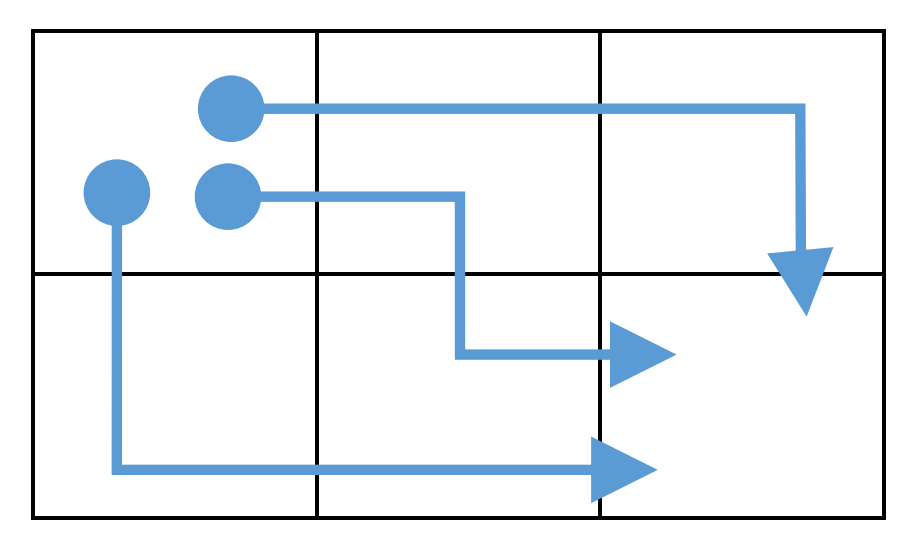
\includegraphics[width=0.5\textwidth]{path.png}
    \caption{路徑問題}
    \label{path}
\end{figure}

我們的問題是計算 $g(m,n)$。定義子問題:以 $g(i,j)$表示出發點走到$(i,j)$的走法數,以矩陣列與行的方式定義位置,出發點為$(1,1)$,終點是$(m,n)$。接著要找出 $g(i,j)$與子問題的遞迴關係,同樣的,我們不必立刻寫出 $g(i,j)$是多少,只要去想,最後一步一定向右或向下,也就是前一個位置一定是$(i,j-1)$或$(i-1,j)$,而且這兩類走法必然不同(沒有重複多算)。根據定義,我們可以得到$g(i,j)=g(i,j-1)+g(i-1,j)\text{ for i>1 and j>1}$;初始條件為$g(i,j)=1(i=1 \text{ or }j=1)$。得到遞迴式之後直接寫遞迴程式就是純遞迴,程式如\autoref{code:path_rec},再一次,遞迴的程式非常沒有效率:
\begin{code}
    \captionof{listing}{路徑問題的遞迴寫法}
    \label{code:path_rec}
    \begin{minted}
#include <iostream>

using namespace std;

long long grid(int m, int n) {
    if (m == 1 || n == 1) return 1;

    return grid(m, n-1) + grid(m-1, n);
}
int main() {
    int m, n;
    cin >> m >> n;
    cout << grid(m, n) << endl;
    return 0;
}

\end{minted}
\end{code}

要把純遞迴改成 DP,就要找計算順序,讓遞迴關係式右邊的出現在左邊的之前,本題的遞迴式為:$g(i,j)=g(i,j-1)+g(i-1,j)$,簡單觀察可以得知,只要 $i$ 與 $j$ 都從小到大就可以滿足需要,所以我們可以採取「由上而下,由左而右」的順序,當然也可以「由左而右,由上而下」,甚至可以沿著 $i+j$ 由小而大的斜線的順序,有點自找苦吃就是了。至於表格,最直覺的方式就是將 $g(i,j)$記錄在一個二維陣列 \texttt{G[i][j]}中。以下是程式,跑得很快,時間複雜度是 $O(mn)$,而遞迴版本的複雜度則是組合數 $\binom{m+n-2}{m-1}$,因為這一題的答案其實有數學解,是排列組合的題目。請不需要擔心數學解這件事,通常程式考試與競賽都不出有數學解的題目,以這題來說,只要將某些格子變成禁止通行或者做一些變化,就難以用數學的方式求解了,畢竟程式考試主要考的是程式技巧。

\begin{code}
    \label{code:path_DP}
    \caption{路徑問題的DP寫法}

    \begin{minted}

#include <iostream>

using namespace std;

int main() {
    long long G[50][50];
    int m, n;
    cin >> m >> n;
    
    for (int i=1; i<=m; i++)
        G[i][1]=1;

    for (int j=1; j<=n; j++)
        G[1][j]=1;

    for (int i=2; i<=m; i++)
        for (int j=2; j<=n; j++)
            G[i][j] = G[i-1][j] + G[i][j-1];

    cout << G[m][n] << endl;

    return 0;
}

\end{minted}
\end{code}
\subsection{狀態轉移}
DP 子問題的遞迴關係式也有人稱為「狀態轉移」,這個名詞大概是從有限狀態機(數位電路設計)來的。子問題可以看成一個狀態,目前的狀態是根據之前的那些狀態,這樣的轉換關係就稱作狀態轉移,設計 DP 時,最重要的就是找出狀態轉移。之前我們將子問題看成「部分解」,所以是在找部分解與更小的解之間的關係,這兩個講法只是描述的方式不一樣,其實是同一回事,有的時候這樣想比較方便,有的時候那樣想比較直覺。雖然我們要在下一章會討論圖(graph),但提到狀態轉移,用圖的術語比較好說明。我們說狀態 A 是狀態 B 的前置狀態(predecessor),如果狀態 B 是由 A 轉移過來的,一個狀態可能有多個前置狀態,通常一個狀態的值是由它的前置狀態的值做某些計算得到。如果我們把每個狀態想像每一個點,若 A 是 B 的前置狀態,則由 A 劃一個箭頭指到 B,我們會得到一個所謂的圖(graph),這個圖就是這個 DP 的狀態轉換圖,在圖論上來說,它必然是個有方向但沒有環路的圖(directed acyclic graph, DAG),所謂環路是指從某點出發,沿著箭頭前進,最後又走到出發點。遞迴關係不會無限遞迴,所以必然沒有環路。我們來看看前面兩個簡單的問題的狀態轉移。小朋友上樓梯問題的子問題是走到第 i 階,關係式 $f(n)=f(n-1)+f(n-2)$,也就是每個狀態由它的前兩個狀態轉移而來。

第二個問題是方格圖的問題,遞迴式是:$g(m,n)=g(m-1,n)+g(m,n-1)$,每一個格子是一個點(狀態),前置狀態是他的左方與上方。

對於一個 DAG,我們一定可以將它的所有點排成某個順序,在此順序中,每個箭頭都由前往後指,也就是說,每個點的前置點都在它之前,這樣的順序稱為拓樸順序(topological sort),我們的 DP 就是要沿著一個拓樸順序來進行。有件事情要提醒,本節說明的狀態轉移以及 DAG 與拓樸順序,是方便思考用的,在DP 解題時通常並不需要把它建出來,也就是建在心中就可以了,不必建在程式中。

\subsection{分類與複雜度}
題目的分類往往有很多種,主要看目的何在而分類,這裡我們以便於理解與學習來分類。一個 DP 如果狀態有 $O(n^x)$而轉移式涉及$O(n^y)$個狀態,一般可稱為 $xDyD$ 的 DP,例如小朋友上樓梯是 $1D0D$ 的,因為有 $n$ 個要算,每次算 $f(i)$只涉及 2 個 $f(i-1)$與 $f(i-2)$。方格路徑的問題則是 $2D0D$,因為有 $n^2$(假設 $m=n$)個要算,每次只需要 2 個(左方與上方)。當然也有一些 DP 不在這個分類中。

一個 $xDyD$ 的 DP,如果沒有優化,很明顯的,時間複雜度就是 $O(n^{x+y})$,一般來說若$y=0$ 時比較簡單,因為遞迴式單純,而且遞迴式找出來時,程式就已經差不多寫完了,因為套個迴圈依序計算就是了。$y=1$ 的 DP 題目通常存在某種優化或需要某些資料結構幫忙,所以會比較難。下一節開始的題目分析,我們的會先介紹 $y=0$,然後再介紹 $y=1$的狀況。

\subsection{Top-down memoization}
前面講到設計 DP 算法的步驟,基本上要先找出遞迴式,然後找出計算順序來避免遞迴。這算是標準的 DP,也稱為 Bottom-up 的 DP。另外有一種實現 DP 的方式是不找計算順序,直接依照遞迴式寫遞迴,但是因為一定要避免遞迴的重複計算,所以採取了一些步驟,這種實現的方式稱為 top-down memoization 的 DP,其中 memoization 字典上應該沒有這個字,大概是為了這個技術自己創造的,這個字是由 memo(備忘錄,便籤小紙條)變來的,這個方法基本上應該是打比賽或重實作的人上發展出來的(偷懶)方法,因為從理論的角度,除了程式好比較寫之外,這麼做沒有好處,但考試與比賽還真的就希望比較好寫。

用比較俏皮的講法,這個方法就是再找到遞迴式之後,直接寫成遞迴版本的程式,但要加上三個動作:

\begin{enumerate}
    \item 開一個表格當作小抄,用來記錄計算過的結果,表格初值設為某個不可能的值,用
          以辨識是否曾經算過。
    \item 在遞迴之前,先偷看一下小抄是否曾經算過,如果小抄上有答案(已經算過),則直
          接回傳答案。
    \item 如果小抄上沒有,就遞迴呼叫,但計算完畢回傳前,要把它記在小抄上。
\end{enumerate}

我們來看看前面介紹的兩個問題的遞迴版本如何改成 top-down DP。\autoref{code:topdown}是熊熊上樓梯,首先注意到它就是拿前面的遞迴版本來改的,修改的部分:第 5 行宣告了一個表格 \texttt{F[]};在遞迴函數中第 8 行做了一個檢查是否 \texttt{F[n]>0} 的動作,如果是則直接回傳,這一題的數字都是正數,所以我們可以用 0 來表示沒算過;如果沒算過,第 9 行就真的遞迴呼叫去計算,然後存在表格中再回傳。


\begin{code}
    \label{code:topdown}
    \caption{熊熊上樓梯的Top-down memoization寫法}
    \begin{minted}

#include <iostream>

using namespace std;

long long F[100] = {0}; // memo, 0 if not computed

long long stair(int n) {
    if (F[n] > 0) return F[n]; // check memo
    F[n] = stair(n-1) + stair(n-2); // record to memo
    return F[n];
}
int main() {
    int n;
    cin >> n;
    F[1]=1, F[2]=2;
    cout << stair(n) << endl;

    return 0;
}
\end{minted}
\end{code}
這個``遞迴"的程式跑的慢不慢呢?基本上跟Bottom-up 跑得一樣神速。我們再來看第二題方格路徑的改法。下面是修改版的程式,其實每一個 top-down 的 DP 幾乎都是長的這個樣子。這裡我們故意用了一些與上一題稍微不同的修改方式,雖然這題也可以用陣列初值為 0 表示沒算過,但我們自己寫陣列的初始化(設為-1),因為有些題目可能有此需要。上一題我們把遞迴終點條件拿掉,替代以在主程式中設定起始點的表格值,這一題我們留著遞迴的終端條件,其實這些差異都不大。這個程式也是跑的跟 Bottom-up 版一樣的神速。

\begin{code}
    \caption{路徑問題的Top-down memoization寫法}
    \begin{minted}
#include <iostream>

using namespace std;

long long G[100][100]; // as memo

long long grid(int m, int n){
    if (m == 1 || n == 1)
        return 1;
    if (G[m][n] >= 0)
        return G[m][n]; // check memo
    // record before return
    return G[m][n] = grid(m, n - 1) + grid(m - 1, n);
}

int main(){
    int m, n;
    cin >> m >> n;
    for (int i = 0; i <= m; i++)
        for (int j = 0; j <= n; j++)
            G[i][j] = -1; // initial unknown
    
    cout << grid(m, n) << endl;

    return 0;
}
\end{minted}
\end{code}

Top-down 的 DP 基本上是個偷懶的方法,我們的建議如下:如果計算順序不難找,還是寫迴圈版,不要過分偷懶,因為遞迴還是有成本與限制,尤其某些系統之下(尤其架在視窗系統下),遞迴的深度有一定的限制,超過限制會導致執行階段的錯誤。在計算順序比較不好找或者比較麻煩時,而且系統是允許的狀況下,就採用 top-down 吧!最常見的情形就是 Tree 的 DP,幾乎參加比賽的選手都寫遞迴的 DFS 版本,因為迴圈版的要找 bottom-up 順序,比較麻煩。不過這裡還是要建議:兩種都要會,可以偷懶的時候才偷懶。
%\chapter{分治 Divide and Conquer}
%\chapter{標頭檔 Headers File}
%\chapter{變數的生命週期}
%\chapter{遞迴 Recursive}
%\chapter{時間複雜度 Time Complexity}
%\chapter{Linked List}
%\chapter{C++ Template}
\end{document}